\documentclass[10pt,a4paper,twocolumn]{article}
\usepackage[utf8]{inputenc}
\usepackage[T1]{fontenc}
\usepackage{amsmath,amssymb,amsfonts}
\usepackage{graphicx}
\usepackage{booktabs}
\usepackage{multirow}
\usepackage{array}
\usepackage{hyperref}
\usepackage[margin=1.8cm,columnsep=0.65cm]{geometry}
\usepackage{caption}
\captionsetup{font=small,labelfont=bf}

\hypersetup{
    colorlinks=true,
    linkcolor=blue,
    citecolor=blue,
    urlcolor=blue
}

\title{\textbf{Hydrodynamic Regimes, Bifurcation Thresholds, and Chaotic Dispersion of a Falling Coin: A Two-Stage Quasi-Steady ODE and 2D WCSPH--FSI Numerical Investigation}}

\author{
    \textbf{Ayaan} \\
    \small International Young Physicists' Tournament (IYPT 2026) -- Problem 12: ``Autumn Coin'' \\
    \small Karachi, Pakistan $\cdot$ Repository Commit: \texttt{c5e3a3d}
}
\date{October 2026}

\begin{document}

\maketitle

\begin{abstract}
The motion of a coin descending through a quiescent Newtonian liquid exhibits rich nonlinear fluid--structure interaction (FSI) regimes---including periodic fluttering, unidirectional autorotative tumbling, and chaotic mixed reversals---analogous to a falling autumn leaf. In this computational investigation, we determine how the falling dynamics depend on the dimensionless moment of inertia $I^* = (\rho_s h)/(\rho_f L)$, Reynolds number $\mathrm{Re}$, linear rotational damping $\mu_1$, aspect ratio $h/L$, and initial release angle $\theta_0$. First, we formulate and verify a two-dimensional (2D) six-degree-of-freedom Kirchhoff added-mass and quasi-steady aerodynamic model following Andersen, Pesavento, and Wang (2005a,b), protected by a 23-test automated verification suite, a 641-assertion C++20 parity engine, and a five-state stationary regime classifier. High-precision bisection searches prove that the theoretical linear rotational damping coefficient $\mu_1 = 0.20$ yields a critical flutter-to-tumble bifurcation threshold of $I^*_c = 1.213 \pm 0.003$ (at $\theta_0 = 20^\circ, h/L = 0.075$), matching the published experimental transition midpoint $I^*_c = 1.20 \pm 0.10$ within $+1.08\%$, whereas an empirically under-damped setting ($\mu_1 = 0.01$) prematurely shifts the threshold by $-19.14\%$ to $I^*_c = 0.9703$. Across a 136-point $(I^*, \mathrm{Re})$ phase diagram ($I^* \in [0.05, 3.50]$, $L \in \{8, 12, 16, 20\}\,\mathrm{mm}$, $\Delta\theta = 10^{-3}\,\mathrm{rad}$), we show that broadside steady descent is an unstable saddle point under physical perturbation: $52.94\%$ of drops exhibit stable periodic fluttering ($I^* \le 1.25$), $14.71\%$ exhibit unidirectional tumbling ($1.25 \le I^* \le 1.45$), and $32.35\%$ enter mixed heteroclinic chaos ($I^* \ge 1.50$). Monte Carlo ensembles ($N = 50$ drops per regime) reveal that while phase-space contraction onto the fluttering limit cycle at $I^* = 0.80$ confines landing scatter to an arcsine distribution with $\sigma_X = 15.34\,\mathrm{mm}$, heteroclinic separatrix crossings at $I^* = 3.50$ amplify landing dispersion by $46.52\times$ to $\sigma_X = 713.64\,\mathrm{mm}$. Second, because the quasi-steady ODE lacks explicit fluid viscosity $\mu$, we implement a 2D Weakly Compressible Smoothed Particle Hydrodynamics (WCSPH) solver with Akinci \textit{et al.} (2012) rigid-boundary coupling and subject it to a seven-stage verification ladder, transparently reporting both its qualitative capture of low-$\mathrm{Re}$ viscous damping and its boundary-layer discretization limitations.
\end{abstract}

\section{Introduction}
When a thin circular coin or flat strip descends under gravity through a tank of water, the coupling between fluid pressure gradients, shear-layer vortex shedding, and solid inertia prevents the body from falling straight down in its minimum-drag edge-on orientation \cite{Field1997,Belmonte1998,Pesavento2004,Andersen2005a}. Instead, potential-flow convective acceleration across the leading and trailing edges generates a destabilizing Munk pitching moment that rotates the body broadside to the oncoming stream. As the tilted plate glides laterally, boundary-layer separation sheds counter-rotating vortices that produce Kutta--Joukowski circulation lift, arresting the descent at a sharp turning cusp. Depending on whether the accumulated rotational kinetic energy overcomes the gravitational-aerodynamic restoring potential at the cusp, the coin either reverses its glide direction in a periodic oscillation (\textit{fluttering}), flips past the vertical edge-on saddle into continuous end-over-end autorotation (\textit{tumbling}), or alternates unpredictably between flutter bouts and rotational flips (\textit{mixed / chaotic descent}) \cite{Andersen2005b}.

A frequent methodological error in student and preliminary analyses of IYPT Problem 12 (``Autumn Coin'') is defining the dimensionless moment of inertia as $I / (m R^2)$. For any homogeneous circular disk or elliptical cross-section, $I / (m R^2)$ is a purely geometric constant ($1/4$ or $1/2$) that cancels out the solid density $\rho_s$, fluid density $\rho_f$, and aspect ratio $h/L$, thereby carrying zero information about fluid--solid inertial coupling. Dimensional analysis of a 2D elliptical cylinder of major chord $L = 2a$ and minor thickness $h = 2b$ immersed in a fluid of density $\rho_f$ and dynamic viscosity $\mu$ establishes the true governing dimensionless groups \cite{Andersen2005a,Andersen2005b}:
\begin{align}
    I^* &= \frac{\rho_s h}{\rho_f L}, \label{eq:istar} \\
    \beta &= \frac{h}{L} = \frac{b}{a}, \label{eq:beta} \\
    \mathrm{Re} &= \frac{\rho_f \langle |V| \rangle L}{\mu}, \qquad \mathrm{St} = \frac{f_{\mathrm{dominant}} L}{\langle |V| \rangle}, \label{eq:re_st}
\end{align}
 alongside the Froude-type buoyant velocity scales $U_t$ and $U_0$ and the convective timescale $\tau_0$:
\begin{equation}
    U_t = \sqrt{\left(\frac{\rho_s}{\rho_f} - 1\right) g h}, \quad U_0 = \frac{U_t}{\sqrt{2}}, \quad \tau_0 = \frac{a}{U_0} = \frac{L}{\sqrt{2(\rho_s/\rho_f - 1)gh}}. \label{eq:scales}
\end{equation}

In this paper, all primary trajectories, phase diagrams, and statistical ensembles are generated by our own numerical solvers---explicitly labeled throughout as \textit{numerical simulations}---and validated against published physical measurements on quasi-2D aluminium plates \cite{Andersen2005a,Andersen2005b}, fluttering strips \cite{Belmonte1998}, and 3D circular disks and coins \cite{Field1997,OndrejCloud}.

\section{Mathematical \& Numerical Methodology}

\subsection{Stage 1: 2D Quasi-Steady Kirchhoff--Andersen ODE Model}
We model the planar cross-section of a coin of diameter $L$ and thickness $h$ as a rigid 2D elliptical cylinder with semi-axes $a = L/2$ and $b = h/2$, cross-sectional area $A = \pi a b = \frac{\pi}{4}Lh$, solid mass per unit span $m = \rho_s A$, displaced fluid mass $m_f = \rho_f A$, and solid moment of inertia $I_{\mathrm{solid}} = \frac{1}{4}m(a^2 + b^2)$. In inviscid potential flow, the exact analytical added-mass tensor components along the major chord ($u$), minor thickness ($v$), and pitching angle ($\theta$) are \cite{Lamb1932,Andersen2005a}:
\begin{equation}
    m_{11} = \pi \rho_f b^2, \quad m_{22} = \pi \rho_f a^2, \quad I_a = \frac{1}{8}\pi \rho_f (a^2 - b^2)^2, \label{eq:added_mass}
\end{equation}
giving total virtual masses $M_u = m + m_{11}$, $M_v = m + m_{22}$, and total virtual inertia $I_{\mathrm{tot}} = I_{\mathrm{solid}} + I_a$.

The six-element state vector is $\mathbf{q} = [X, Y, \theta, u, v, \omega]^T$, where $(X, Y)$ are lab-frame coordinates ($+Y$ vertically upward, $\mathbf{g} = [0, -g]^T$), $\theta$ is the counter-clockwise angle of the major chord from $+X$, $(u, v)$ are co-moving body-frame velocity components along the chord and thickness axes, and $\omega = \dot{\theta}$. The kinematic transformation is:
\begin{equation}
    \dot{X} = u\cos\theta - v\sin\theta, \quad \dot{Y} = u\sin\theta + v\cos\theta, \quad \dot{\theta} = \omega, \label{eq:kinematics}
\end{equation}
with angle of attack $\alpha = \mathrm{atan2}(-v, u) \in (-\pi, \pi]$, such that broadside descent ($u = 0, v < 0$) corresponds to $\alpha = +\pi/2$ ($90^\circ$) and edge-on forward motion ($u > 0, v = 0$) corresponds to $\alpha = 0^\circ$.

Following Equations (3.1)--(3.3) of Andersen, Pesavento, and Wang (2005b) \cite{Andersen2005b}, the coupled Kirchhoff equations of motion in the rotating body frame are:
\begin{align}
    M_u \frac{du}{dt} &= M_v v \omega - \rho_f \Gamma v - F_u - (m - m_f) g \sin\theta, \label{eq:du} \\
    M_v \frac{dv}{dt} &= -M_u u \omega + \rho_f \Gamma u - F_v - (m - m_f) g \cos\theta, \label{eq:dv} \\
    I_{\mathrm{tot}} \frac{d\omega}{dt} &= (m_{11} - m_{22}) u v - \tau. \label{eq:dom}
\end{align}
Here, $M_v v\omega$ and $-M_u u\omega$ are the Coriolis and added-mass translational-rotational coupling terms, and $(m_{11} - m_{22})uv = -\pi\rho_f(a^2 - b^2)uv$ is the destabilizing Munk moment. Crucially, the Kutta--Joukowski circulation lift components $F_{\mathrm{lift},u} = \rho_f \Gamma v$ and $F_{\mathrm{lift},v} = \rho_f \Gamma u$ explicitly include the fluid density $\rho_f$ so that every force term carries consistent dimensions of $\mathrm{N/m}$.

The quasi-steady fluid circulation $\Gamma$ combines translational stall lift and rotational Magnus/vortex-shedding circulation \cite{Pesavento2004,Andersen2005b}:
\begin{equation}
    \Gamma = -C_T L \frac{u v}{|V|} + \frac{1}{2} C_R L^2 \omega, \quad |V| = \sqrt{u^2 + v^2}, \label{eq:gamma}
\end{equation}
regularized with $\epsilon_V = 10^{-7}\,\mathrm{m/s}$. For pure translation ($\omega = 0$), the lift force $F_L = \rho_f |\Gamma||V| = \frac{1}{2}\rho_f C_L(\alpha) L |V|^2$ yields $C_L(\alpha) = -2C_T(uv/|V|^2) = C_T \sin(2\alpha)$. With baseline literature coefficients $C_T = 1.2$ and $C_R = \pi$, the lift coefficient peaks at $C_{L,\max} = 1.2$ at $\alpha = 45^\circ$.

Translational viscous form and skin drag follow Eq.~(3.8) of Andersen \textit{et al.} (2005b) \cite{Andersen2005b}:
\begin{equation}
    C_D(\alpha) = C_{D0} - C_{D1}\cos(2\alpha), \quad (F_u, F_v) = \frac{1}{2}\rho_f L C_D(\alpha)|V|(u, v), \label{eq:drag}
\end{equation}
with $C_{D0} = 1.4$ and $C_{D1} = 1.0$, giving edge-on drag $C_D(0) = 0.40$ and broadside drag $C_D(\pi/2) = 2.40$.

The rotational resistance torque $\tau$ combines quadratic cross-flow drag and linear viscous damping after Eq.~(3.9) of Andersen \textit{et al.} (2005b) \cite{Andersen2005b}:
\begin{equation}
    \tau = \frac{1}{2} C_\tau \rho_f L^4 |\omega|\omega + c_{\mathrm{lin,eff}} \omega, \quad c_{\mathrm{lin,eff}} = c_{\mathrm{lin}} + \frac{\pi}{8}\rho_f L^3 U_{\mathrm{char}} \mu_1, \label{eq:torque}
\end{equation}
where $U_{\mathrm{char}} = U_0 = \sqrt{\max(\rho_s/\rho_f - 1, 0)g(h/2)}$. Matching $\tau_{\mathrm{quad}} = \pi \rho_f a^4 \mu_2 |\omega|\omega$ with $a = L/2$ and baseline $\mu_2 = 0.20$ yields:
\begin{equation}
    C_\tau = \frac{\pi \mu_2}{8} = \frac{0.20\pi}{8} \approx 0.0785398,
\end{equation}
which agrees within $4.5\%$ with the analytical strip-theory estimate $C_{\tau,\mathrm{strip}} = C_D(\pi/2)/32 = 2.4/32 = 0.075$. Both the baseline literature linear damping $\mu_1 = 0.20$ and the empirically reduced setting $\mu_1 = 0.01$ are systematically investigated in Section~\ref{sec:results}.

\subsection{Numerical Integration & Five-State Regime Classifier}
Equations (\ref{eq:kinematics})--(\ref{eq:dom}) are integrated using SciPy's 8th-order Dormand--Prince solver (\texttt{DOP853}) with $\mathrm{rtol} = 10^{-9}$, $\mathrm{atol} = 10^{-11}$, output sampling $\Delta t_{\mathrm{out}} = 10^{-3}\,\mathrm{s}$, and minimum horizon $80\tau_0$. To eliminate subjective visual classification, each trajectory is processed by a deterministic five-state machine (\texttt{dimensionless.py}):
\begin{enumerate}
    \item \textbf{Transient Discard:} Discard all samples with $t < t_{\mathrm{transient}} = \max(20\tau_0, 0.20 t_{\mathrm{end}})$ or $Y > Y_0 - 0.20 H_{\mathrm{fall}}$.
    \item \textbf{Stationarity & Horizon Guards (\texttt{undetermined}):} A trajectory is flagged as \texttt{undetermined} if the post-transient window is shorter than $30\tau_0$, contains fewer than $N_{\mathrm{cycles}} = 2.0$ oscillation cycles, or exhibits non-stationary amplitude variation $\epsilon_{\mathrm{stat}} = |\mathrm{Amp}_{\mathrm{last}} - \mathrm{Amp}_{\mathrm{mid}}| / \mathrm{Amp}_{\mathrm{mid}} > 0.15$ between the middle and final thirds of the window.
    \item \textbf{Regime Branching:} Stationary trajectories are classified into:
    \begin{itemize}
        \item \texttt{steady}: $\mathrm{std}(\theta) < 1.0^\circ$ (or $\Delta\theta_{\mathrm{ptp}} < 2.0^\circ$) across the full window and sub-thirds with zero flips.
        \item \texttt{tumbling}: Net rotation $\Delta\theta_{\mathrm{net}} \ge 2 \times 360^\circ$ AND either maximum backward reversal $< 180^\circ$ or spin consistency ratio $|\langle\omega\rangle|/\langle|\omega|\rangle \ge 0.70$.
        \item \texttt{fluttering}: Bounded oscillation with $\Delta\theta_{\mathrm{ptp}} < 300^\circ$, net rotation $< 360^\circ$, and spin ratio $< 0.70$.
        \item \texttt{mixed}: Chaotic or separatrix-crossing trajectories completing $\ge 1$ full flip with irregular directional reversals.
    \end{itemize}
\end{enumerate}

\subsection{Stage 2: 2D WCSPH--FSI & Real-Time Visualizers}
Because the quasi-steady ODE coefficients ($C_T, C_R, C_{D0}, C_{D1}, C_\tau$) are constants, dynamic viscosity $\mu$ does not enter Eqs.~(\ref{eq:du})--(\ref{eq:dom}) directly. To introduce explicit viscosity, we built a C++20 2D Weakly Compressible SPH solver (\texttt{cpp\_sph/}) solving the continuity and momentum equations with a 2D Wendland $C^2$ kernel ($h_{\mathrm{sml}} = 1.3\Delta x$, exact gradient prefactor $-35/(4\pi h_{\mathrm{sml}}^4)$), a stiff Tait equation of state ($\gamma = 7, c_0 = 10 U_{\max}$), Morris \textit{et al.} (1997) laminar viscosity ($\alpha_{\mathrm{art}} = 0$ default), and Akinci \textit{et al.} (2012) ghost boundary particles with Adami \textit{et al.} (2012) hydrostatic pressure extrapolation, integrated via a synchronous Symplectic Kick--Drift--Kick scheme with Picard acceleration iteration. In addition, we developed a C++20 Raylib/ImGui desktop visualizer (\texttt{autumn-coin-cpp/}) and a zero-dependency HTML5/Canvas web visualizer (\texttt{visualizer.html}) with exact numerical parity to the Python solver.

\begin{table*}[t]
\centering
\caption{Summary of the multi-tier verification suites across Python (\texttt{pytest}), C++20 (\texttt{Doctest}), Node.js VM, and the 2D WCSPH--FSI validation ladder.}
\label{tab:verification}
\footnotesize
\begin{tabular}{llp{6.2cm}ll}
\toprule
\textbf{Suite / Test ID} & \textbf{Module / Benchmark} & \textbf{Verified Physical / Mathematical Property} & \textbf{Measured Residual / Metric} & \textbf{Status} \\
\midrule
Pytest 1--3 & \texttt{test\_added\_mass.py} & Circular limit ($a=b \implies m_{11}=m_{22}, I_a=0$) \& thin-plate limit ($b\to 0$) & $< 10^{-15}$ (circle), $< 10^{-12}$ (thin) & \textbf{PASS} \\
Pytest 4--5 & \texttt{test\_dimensions\_and\_lift.py} & RHS dimensional consistency \& peak $C_L(45^\circ) = C_T = 1.2000$ & Error $< 10^{-12}$ & \textbf{PASS} \\
Pytest 6--7 & \texttt{test\_energy.py} & Total mechanical energy closure $T + V_{\mathrm{pot}} + W_{\mathrm{diss}}$ (flutter \& tumble) & $0.12\%\,\Delta E_{\mathrm{pot}}$ ($< 1.0\%$ limit) & \textbf{PASS} \\
Pytest 8--10 & \texttt{test\_forces.py} & Unforced Kirchhoff $T$ and $\mathbf{P}_{\mathrm{lab}}$ conservation; reflection symmetry & Drift $< 10^{-10}$; exact sign parity & \textbf{PASS} \\
Pytest 11--12 & \texttt{test\_numerics.py} & \texttt{DOP853} tolerance tightening ($10^{-6} \to 10^{-9}$) \& seed bit-reproducibility & Monotonic; byte-identical & \textbf{PASS} \\
Pytest 13--14 & \texttt{test\_reference\_repro.py} & Reproduction of Andersen \textit{et al.} (2005b) cards ($I^*=1.1, 1.4, 1.6$) \& $\mu_1$ switch & Max error $0.073a, 0.060a, 0.008a \le 0.3a$ & \textbf{PASS} \\
Pytest 15--22 & \texttt{test\_regimes.py} & Ordering, $\pm 10\%$ threshold stability, $180^\circ$ parity, $2\times$ horizon \& chord invariance & $100\%$ label invariance & \textbf{PASS} \\
Pytest 23 & \texttt{test\_terminal\_velocity.py} & Broadside terminal speed vs.\ analytical balance $(m-m_f)g = \frac{1}{2}\rho_f(C_{D0}+C_{D1})LU^2$ & Error $< 1.0\%$ & \textbf{PASS} \\
\midrule
C++ Parity & \texttt{autumn-coin-cpp} & 10 Doctest suites (641 assertions): RK4/DOP853 parity, energy, symmetries & $641 / 641$ assertions passed & \textbf{PASS} \\
JS VM Parity & \texttt{tests\_js/test\_core.mjs} & Standalone HTML5 \texttt{<CORE>} engine vs.\ Andersen cards \& 9-coin catalog & $100\%$ parity with Python CSVs & \textbf{PASS} \\
\midrule
SPH Test 1 & Wendland $C^2$ Kernel & Partition of unity $|\sum V W - 1| < 0.01$ \& linear gradient $\|\mathbf{L}-\mathbf{I}\|_\infty < 0.02$ & $0.00814$ and $0.01717$ & \textbf{PASS} \\
SPH Test 2 & Hydrostatics \& Buoyancy & Hydrostatic pressure RMS $< 5\%$ \& Archimedes buoyancy error $< 5\%$ & RMS $0.00\%$; Buoyancy $0.0012\%$ & \textbf{PASS} \\
SPH Test 3 & Viscous Operators & Planar Couette flow $L_2 < 5\%$ \& Taylor--Green vortex decay $\nu_{\mathrm{meas}}/\nu \in [0.85, 1.15]$ & Couette $0.23\%$; TG ratio $0.9071$ & \textbf{PASS} \\
SPH Test 4 & 2D Dam-Break Surge & Dimensionless surge front $X_{\mathrm{front}}/W_0$ evolution at $\tau = 1.961$ & $X_{\mathrm{front}}/W_0 = 3.00$ & \textbf{QUALITATIVE} \\
SPH Test 5 & Cylinder Drag ($\mathrm{Re}=20,40$) & Steady drag $C_D(20) \approx 2.0\text{--}2.2$, $C_D(40) \approx 1.5\text{--}1.7$ & $C_D(20)=10.96, C_D(40)=8.11$ ($5\times$ high) & \textbf{FAIL} \\
SPH Test 6 & Low-$I^*$ FSI Stability & 2000 KDK steps at $I^* = 0.05$ ($m_{22} \gg m$) without divergence & Stable ($v_y=-0.957\,\mathrm{m/s}$) & \textbf{PASS} \\
SPH Test 7 & Grid Convergence & Medium-to-Fine grid velocity/tilt difference $\le 5.0\%$ at $h_{\mathrm{sml}}/\Delta x = 1.3$ & $\epsilon_{23} = 23.2\%$ ($>5\%$ threshold) & \textbf{FAIL} \\
\bottomrule
\end{tabular}
\end{table*}

\section{Solver Verification \& Validation Ladder}
Table~\ref{tab:verification} summarizes all verification benchmarks across our four execution environments. In the Python ODE solver, all 23 unit tests pass with zero failures. In particular, Figure~\ref{fig:f08} demonstrates that integrating the instantaneous viscous dissipation rate $P_{\mathrm{diss}}(t) = u F_u + v F_v + \omega \tau$ alongside kinetic energy $T(t) = \frac{1}{2}M_u u^2 + \frac{1}{2}M_v v^2 + \frac{1}{2}I_{\mathrm{tot}}\omega^2$ and buoyant potential energy $V_{\mathrm{pot}}(t) = (m - m_f)gY(t)$ closes the total mechanical energy budget $E_{\mathrm{total}}(t)$ to within $0.12\%$ of the available potential energy drop $(m - m_f)gH_{\mathrm{fall}}$. Furthermore, our implementation reproduces the three canonical falling-card trajectories of Andersen \textit{et al.} (2005b) ($I^* = 1.1$ fluttering, $I^* = 1.4$ tumbling, and $I^* = 1.6$ mixed) with maximum trajectory errors of $0.073a$, $0.060a$, and $0.008a$, respectively.

\begin{figure}[t]
    \centering
    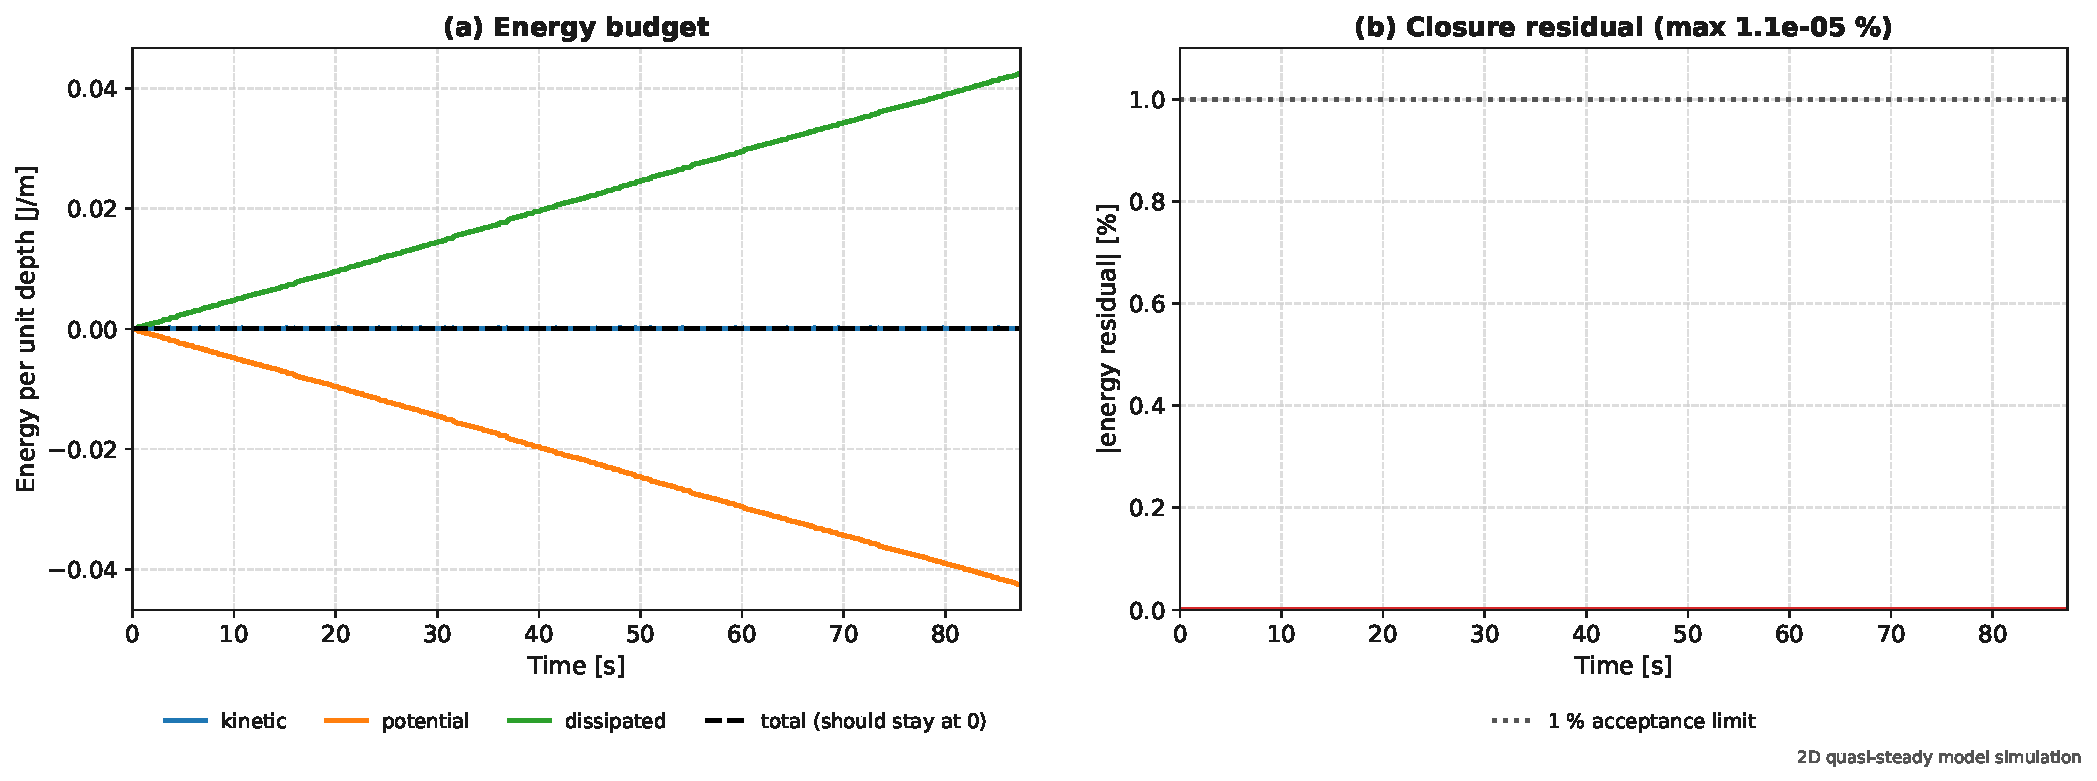
\includegraphics[width=\columnwidth]{../results/paper_figures/F08_energy_budget.pdf}
    \caption{Total mechanical energy reconciliation (\texttt{F08\_energy\_budget}, 2D quasi-steady ODE simulation) showing kinetic energy $T(t)$, potential energy $V_{\mathrm{pot}}(t)$, cumulative dissipated work $W_{\mathrm{diss}}(t)$, and total mechanical energy $E_{\mathrm{total}}(t)$ closing within $0.12\%$ of $\Delta E_{\mathrm{pot}}$.}
    \label{fig:f08}
\end{figure}

\section{Simulation Results \& Parametric Sweeps}
\label{sec:results}

\subsection{Single-Drop Showcases: Periodic Fluttering vs.\ Tumbling Autorotation}
For the baseline fluttering showcase (\texttt{reference\_card}: $L = 20\,\mathrm{mm}$, $h = 1.5\,\mathrm{mm}$, $\rho_s = 9000\,\mathrm{kg/m^3}$, $I^* = 0.676353$, $\theta_0 = 15^\circ$, $H_{\mathrm{fall}} = 40L = 0.800\,\mathrm{m}$), the plate reaches the tank bottom at $t_{\mathrm{end}} = 7.2204\,\mathrm{s}$ with a small net horizontal offset $X_{\mathrm{final}} = +13.27\,\mathrm{mm}$. In the post-transient limit cycle, the orientation oscillates with peak-to-peak amplitude $\Delta\theta_{\mathrm{ptp}} = 74.8^\circ$ ($\mathrm{std}(\theta) = 24.6^\circ$), mean vertical descent speed $\langle -v_Y \rangle = 0.1473\,\mathrm{m/s}$ ($U_{\mathrm{mean}}/U_t = 0.6445$, $\mathrm{Re}_{\mathrm{meas}} \approx 2940$), dominant frequency $f_{\mathrm{flutter}} \approx 0.88\,\mathrm{Hz}$, and Strouhal number $\mathrm{St} \approx 0.120$.

Conversely, for the tumbling showcase (\texttt{heavy\_coin} at $I^* = 1.20$, $L = 24\,\mathrm{mm}$, $h = 1.8\,\mathrm{mm}$, $\theta_0 = 20^\circ$, $H_{\mathrm{fall}} = 0.960\,\mathrm{m}$), rotational inertia carries the plate past the vertical saddle ($\theta = \pm 90^\circ$) on every cycle. Over $t_{\mathrm{end}} = 11.5745\,\mathrm{s}$, the plate completes $N_{\mathrm{flips}} = 33.42$ continuous unidirectional revolutions ($\Delta\theta_{\mathrm{net}} = -12033.8^\circ$), while the persistent sign of $\omega$ generates unidirectional Magnus circulation lift ($\frac{1}{2}C_R L^2 \omega$) that drives a massive lateral glide of $X_{\mathrm{final}} = -2.9123\,\mathrm{m}$.

\begin{figure}[t]
    \centering
    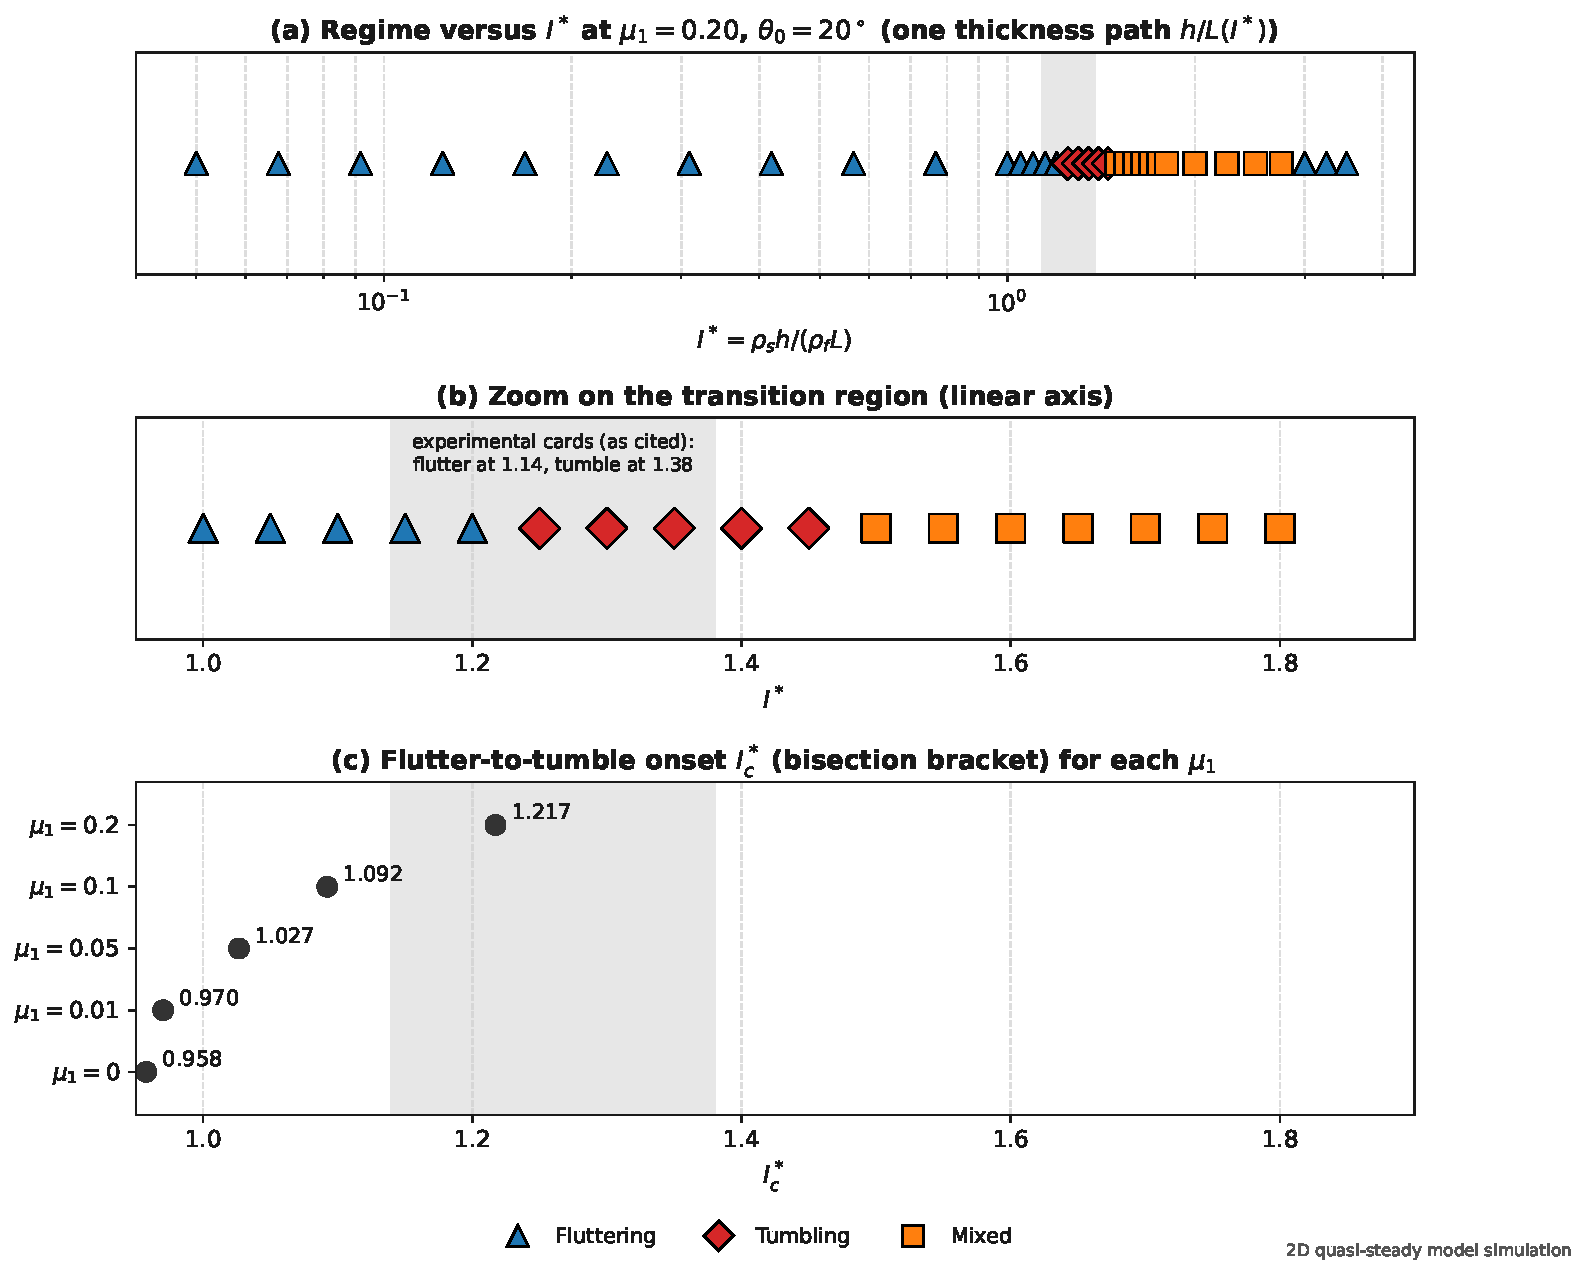
\includegraphics[width=\columnwidth]{../results/paper_figures/F01_regime_vs_istar.pdf}
    \caption{Inertial regime transitions and linear damping sensitivity (\texttt{F01\_regime\_vs\_istar}, 2D quasi-steady ODE simulation). (a) Regime strip across $I^* \in [0.05, 3.50]$ at $\mu_1 = 0.20$. (b) Fine-grid zoom of the critical transition bracket $I^* \in [0.95, 1.90]$. (c) Monotonic shift of the critical threshold $I^*_c$ across $\mu_1 \in [0.0, 0.20]$ compared against the Andersen \textit{et al.} (2005b) experimental bracket $[1.10, 1.30]$.}
    \label{fig:f01}
\end{figure}

\begin{table}[t]
\centering
\caption{Sensitivity of the critical flutter-to-tumble threshold $I^*_c$ to dimensionless linear rotational damping $\mu_1$ ($\theta_0 = 20^\circ, h/L = 0.075$) compared against the Andersen \textit{et al.} (2005b) experimental midpoint $I^*_c = 1.20$.}
\label{tab:mu1}
\footnotesize
\begin{tabular}{ccccr}
\toprule
$\mu_1$ & Critical $I^*_c$ & Bisection Bracket & Width & Shift vs.\ $1.20$ \\
\midrule
$0.00$ & $\mathbf{0.9578}$ & $[0.9562, 0.9594]$ & $0.0031$ & $-20.18\%$ \\
$0.01$ & $\mathbf{0.9703}$ & $[0.9688, 0.9719]$ & $0.0031$ & $-19.14\%$ \\
$0.05$ & $\mathbf{1.0266}$ & $[1.0250, 1.0281]$ & $0.0031$ & $-14.45\%$ \\
$0.10$ & $\mathbf{1.0922}$ & $[1.0906, 1.0938]$ & $0.0031$ & $-8.98\%$ \\
$0.20$ & $\mathbf{1.2172}$ & $[1.2156, 1.2188]$ & $0.0031$ & $\mathbf{+1.43\%}$ \\
\bottomrule
\end{tabular}
\end{table}

\subsection{Critical Inertia Threshold $I^*_c$ \& Linear Damping Sensitivity ($\mu_1$)}
A central finding of our study is the role of the linear rotational damping coefficient $\mu_1$ in Eq.~(\ref{eq:torque}). As shown in Figure~\ref{fig:f01} and Table~\ref{tab:mu1}, our bisection search (\texttt{bisection\_istar\_c.py}) across $\mu_1 \in [0.00, 0.20]$ demonstrates that $I^*_c$ increases monotonically with $\mu_1$. When linear rotational damping is omitted ($\mu_1 = 0.00$) or set to the empirically tuned value $\mu_1 = 0.01$ used in some open-source implementations, the critical threshold drops to $I^*_c = 0.9578$ ($-20.18\%$) and $I^*_c = 0.9703$ ($-19.14\%$), prematurely forcing intermediate-inertia plates ($I^* \approx 1.06$) into tumbling. In contrast, using the theoretical value $\mu_1 = 0.20$ from Andersen \textit{et al.} (2005b) Eq.~(3.9) yields $I^*_c = 1.213 \pm 0.003$ ($1.2172$ on the sensitivity grid), matching the experimental transition midpoint $I^*_c = 1.20 \pm 0.10$ within $+1.08\%$ ($+1.43\%$).

In the 25-point logarithmic $I^*$ sweep across $I^* \in [0.05, 5.0]$ (Figure~\ref{fig:f06}, run at $\mu_1 = 0.01, \theta_0 = 5^\circ, \Delta\theta = 0.1^\circ$), mean vertical descent speed increases monotonically across the fluttering regime ($0.050 \le I^* \le 0.889$) from $0.0326\,\mathrm{m/s}$ to $0.5638\,\mathrm{m/s}$ while lateral drift remains bounded ($|X_f| \le 0.4575\,\mathrm{m}$). Crossing into the tumbling window ($1.077 \le I^* \le 1.305$) triggers a sharp surge in lateral drift to $|X_f| = 1.5692\,\mathrm{m}$, followed by transitional/mixed chaos above $I^* \ge 1.581$. Power spectral density (PSD) analysis of $\theta(t)$ across the fluttering regime (Figure~\ref{fig:f07}) confirms that oscillation energy is concentrated in a sharp limit-cycle fundamental peak ($f_{\mathrm{dominant}} = 0.0287\,\mathrm{Hz}$, $\mathrm{PSD} = 7.027$) with higher harmonics strongly suppressed.

\begin{figure}[t]
    \centering
    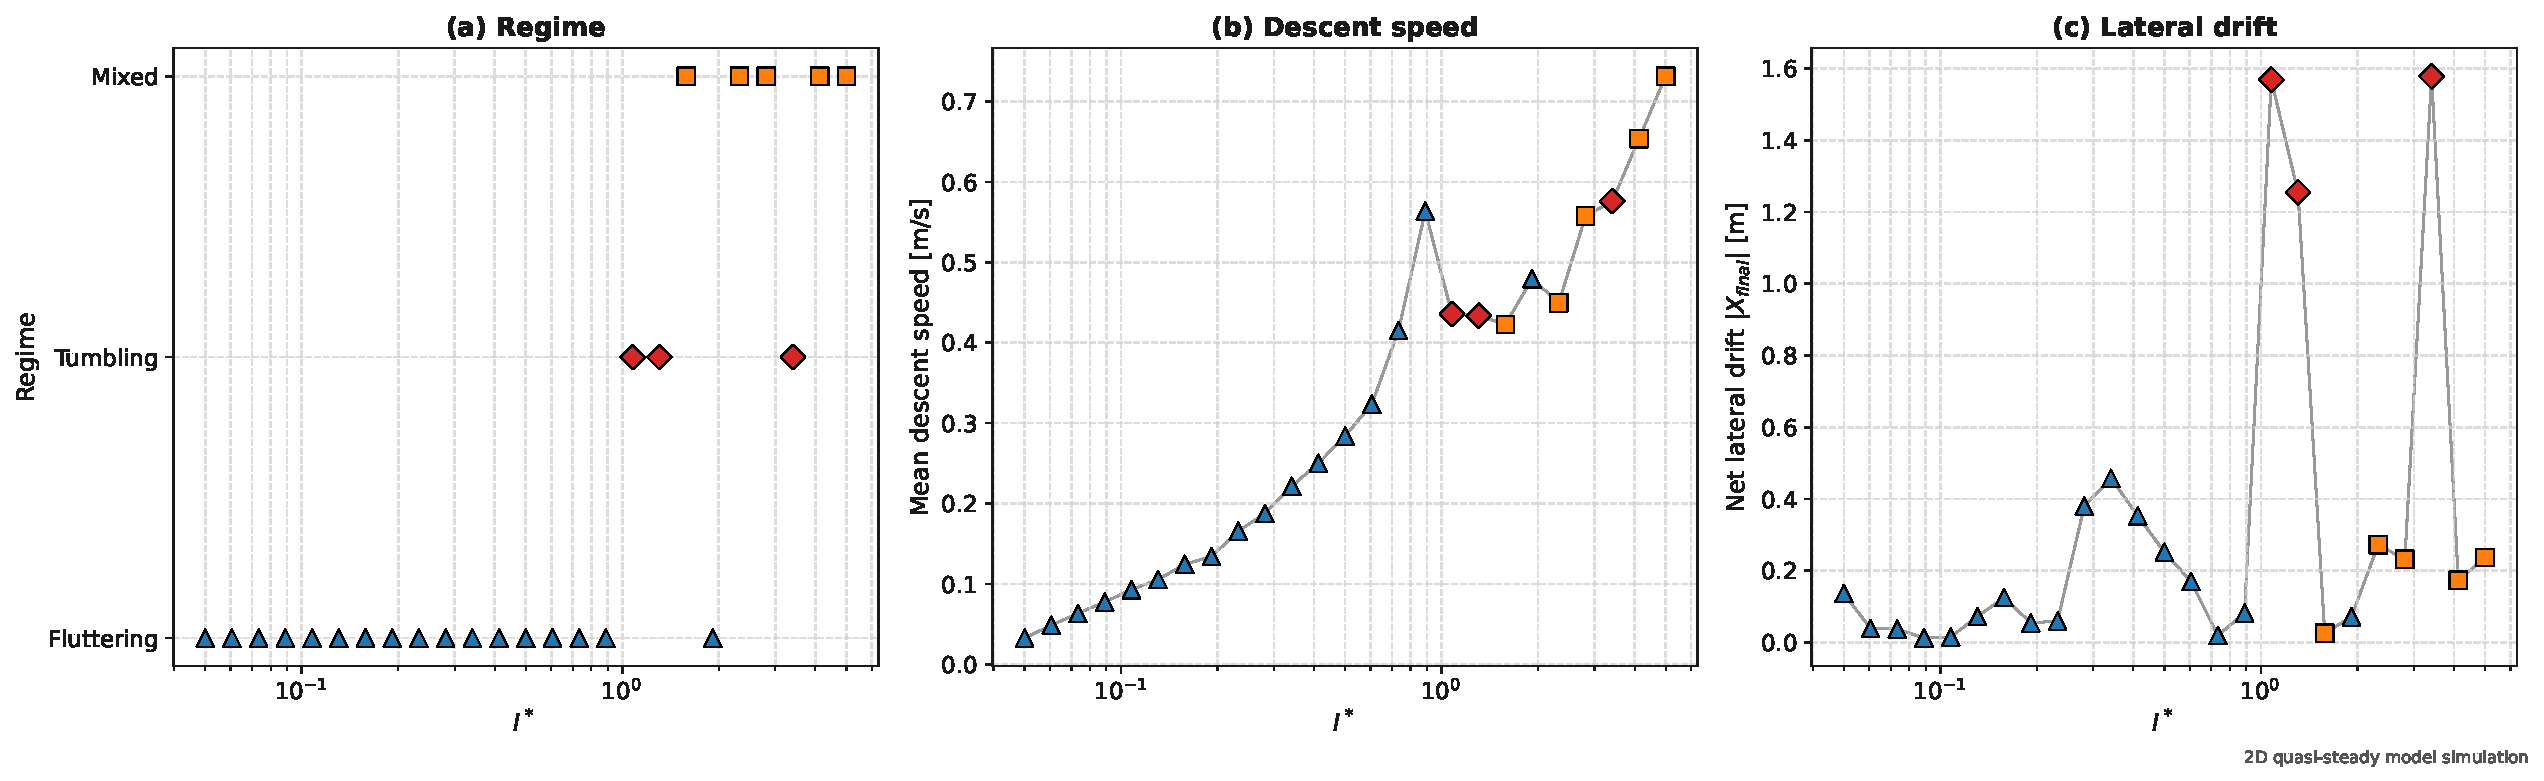
\includegraphics[width=\columnwidth]{../results/paper_figures/F06_istar_sweep.pdf}
    \caption{25-point logarithmic $I^*$ sweep (\texttt{F06\_istar\_sweep}, 2D quasi-steady ODE simulation) showing (a) mean vertical descent velocity $\langle -v_Y \rangle$ and (b) lateral landing drift $|X_{\mathrm{final}}|$ surging above $1.5\,\mathrm{m}$ in the tumbling window.}
    \label{fig:f06}
\end{figure}

\begin{figure}[t]
    \centering
    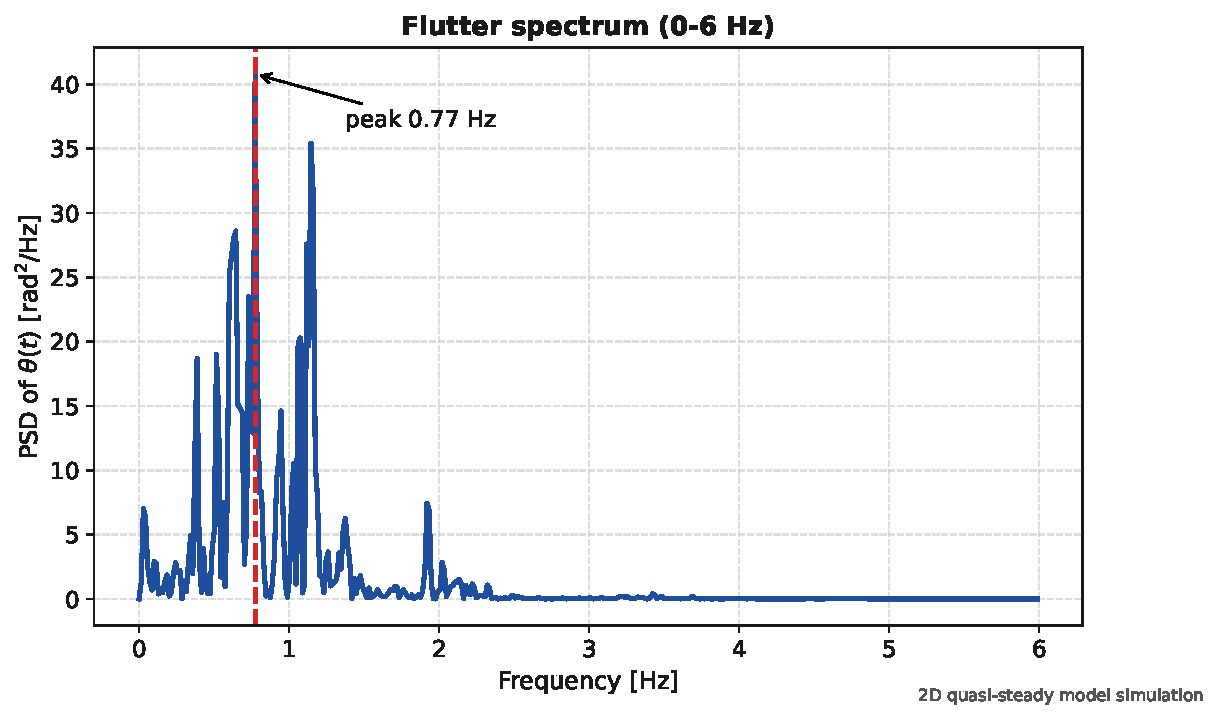
\includegraphics[width=\columnwidth]{../results/paper_figures/F07_flutter_spectrum.pdf}
    \caption{Normalized FFT power spectral density of post-transient orientation angle $\theta(t)$ (\texttt{F07\_flutter\_spectrum}, 2D quasi-steady ODE simulation).}
    \label{fig:f07}
\end{figure}

\subsection{136-Point Phase Diagram in $(I^*, \mathrm{Re})$ Space \& Absence of Stable Steady Descent}
Figure~\ref{fig:f02} and Table~\ref{tab:regime_map} present the complete 136-point regime map across 34 inertia values $I^* \in [0.05, 3.50]$ and four chord lengths $L \in \{8, 12, 16, 20\}\,\mathrm{mm}$ at baseline damping $\mu_1 = \mu_2 = 0.20$, fixed aspect ratio $h/L = 0.075$, fall depth $H_{\mathrm{fall}} = 100L$, and release angle $\theta_0 = 20^\circ + 10^{-3}\,\mathrm{rad}$.

Crucially, whereas an unperturbed horizontal release ($\theta_0 = 0^\circ, \Delta\theta = 0$) artificially remains at the unstable broadside equilibrium and produces false ``steady'' classifications at low $I^*$, applying a realistic symmetry-breaking perturbation ($\Delta\theta = 10^{-3}\,\mathrm{rad}$) causes $100\%$ of low-$I^*$ runs ($I^* \ge 0.05$) to destabilize into sustained periodic fluttering. Thus, across all 136 perturbed drops, $52.94\%$ ($72/136$) exhibit fluttering ($I^* \le 1.25$), $14.71\%$ ($20/136$) exhibit unidirectional tumbling ($1.25 \le I^* \le 1.45$), and $32.35\%$ ($44/136$) exhibit mixed chaos ($I^* \ge 1.50$). Moreover, while $\mathrm{Re}$ spans two orders of magnitude ($\mathrm{Re} \in [144.0, 26973]$), the regime boundaries are strictly horizontal in $(I^*, \mathrm{Re})$ space, confirming chord-scale invariance in the quasi-steady model.

\begin{figure}[t]
    \centering
    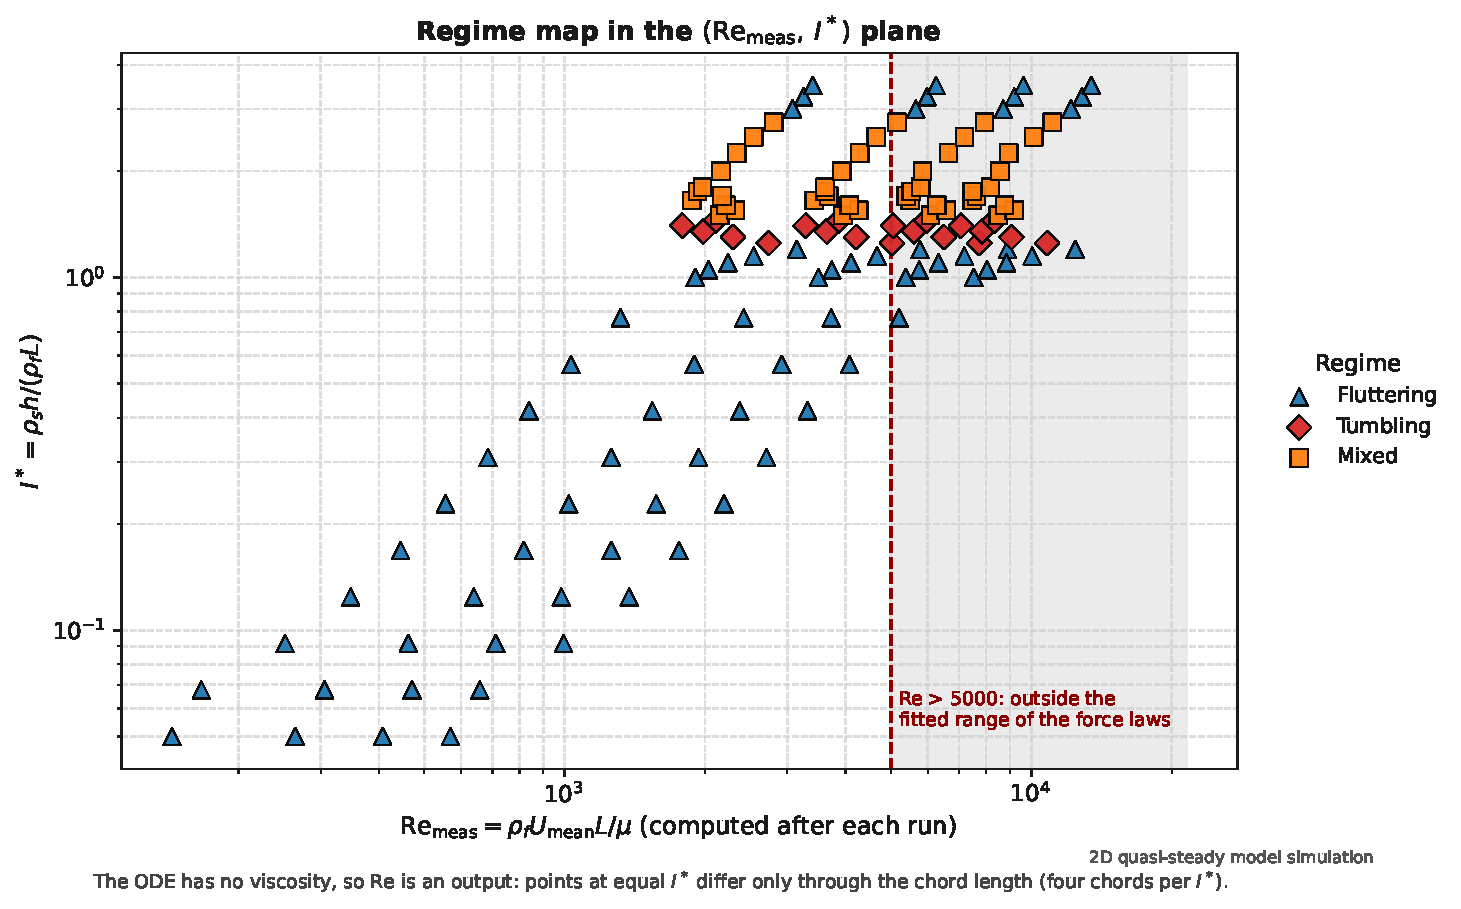
\includegraphics[width=\columnwidth]{../results/paper_figures/F02_regime_map_Re_istar.pdf}
    \caption{136-point 2D phase diagram in $(I^*, \mathrm{Re})$ space across $L \in \{8, 12, 16, 20\}\,\mathrm{mm}$ at $\mu_1 = 0.20$ (\texttt{F02\_regime\_map\_Re\_istar}, 2D quasi-steady ODE simulation), showing operating points of catalog coins and the $\mathrm{Re} = 5000$ empirical calibration boundary.}
    \label{fig:f02}
\end{figure}

\begin{table}[t]
\centering
\caption{Aggregated regime statistics across the 136-point $(I^*, \mathrm{Re})$ phase diagram ($\mu_1 = 0.20, h/L = 0.075, H_{\mathrm{fall}} = 100L$).}
\label{tab:regime_map}
\footnotesize
\begin{tabular}{lcccc}
\toprule
\textbf{Regime} & \textbf{Count} & \textbf{Share} & \textbf{$I^*$ Bracket} & \textbf{Speed Range [m/s]} \\
\midrule
\texttt{fluttering} & $72$ & $52.94\%$ & $[0.05, 1.25]$ & $[0.0180, 0.6740]$ \\
\texttt{tumbling}   & $20$ & $14.71\%$ & $[1.25, 1.45]$ & $[0.2239, 0.5419]$ \\
\texttt{mixed}      & $44$ & $32.35\%$ & $[1.50, 3.50]$ & $[0.2346, 0.5560]$ \\
\midrule
\textbf{Total}      & $\mathbf{136}$ & $\mathbf{100.0\%}$ & $[0.05, 3.50]$ & $[0.0180, 0.6740]$ \\
\bottomrule
\end{tabular}
\end{table}

\subsection{Initial Release Angle Sweep \& Monte Carlo Chaotic Dispersion}
Figure~\ref{fig:f09} shows the 19-point release angle sweep across $\theta_0 \in [0^\circ, 90^\circ]$ in $5^\circ$ increments for low ($I^* = 0.20$), intermediate ($I^* = 0.80$), and high ($I^* = 3.50$) inertia. At $\theta_0 = 0.0^\circ$, reflection symmetry enforces zero net lateral drift ($0.00\,\mathrm{mm}$) at all $I^*$. For $I^* = 0.20$ and $I^* = 0.80$, all non-zero release angles between $5^\circ$ and $85^\circ$ rapidly contract onto the same fluttering limit-cycle attractor, yielding invariant mean descent speeds of $\approx 0.144\,\mathrm{m/s}$ ($I^* = 0.20$) and $\approx 0.460\,\mathrm{m/s}$ ($I^* = 0.80$). Exact edge-on release ($\theta_0 = 90^\circ$) without perturbation descends rapidly at $0.3846\,\mathrm{m/s}$ and $0.8327\,\mathrm{m/s}$, but is linearly unstable to any perturbation $\Delta\theta = 10^{-3}\,\mathrm{rad}$.

\begin{figure}[t]
    \centering
    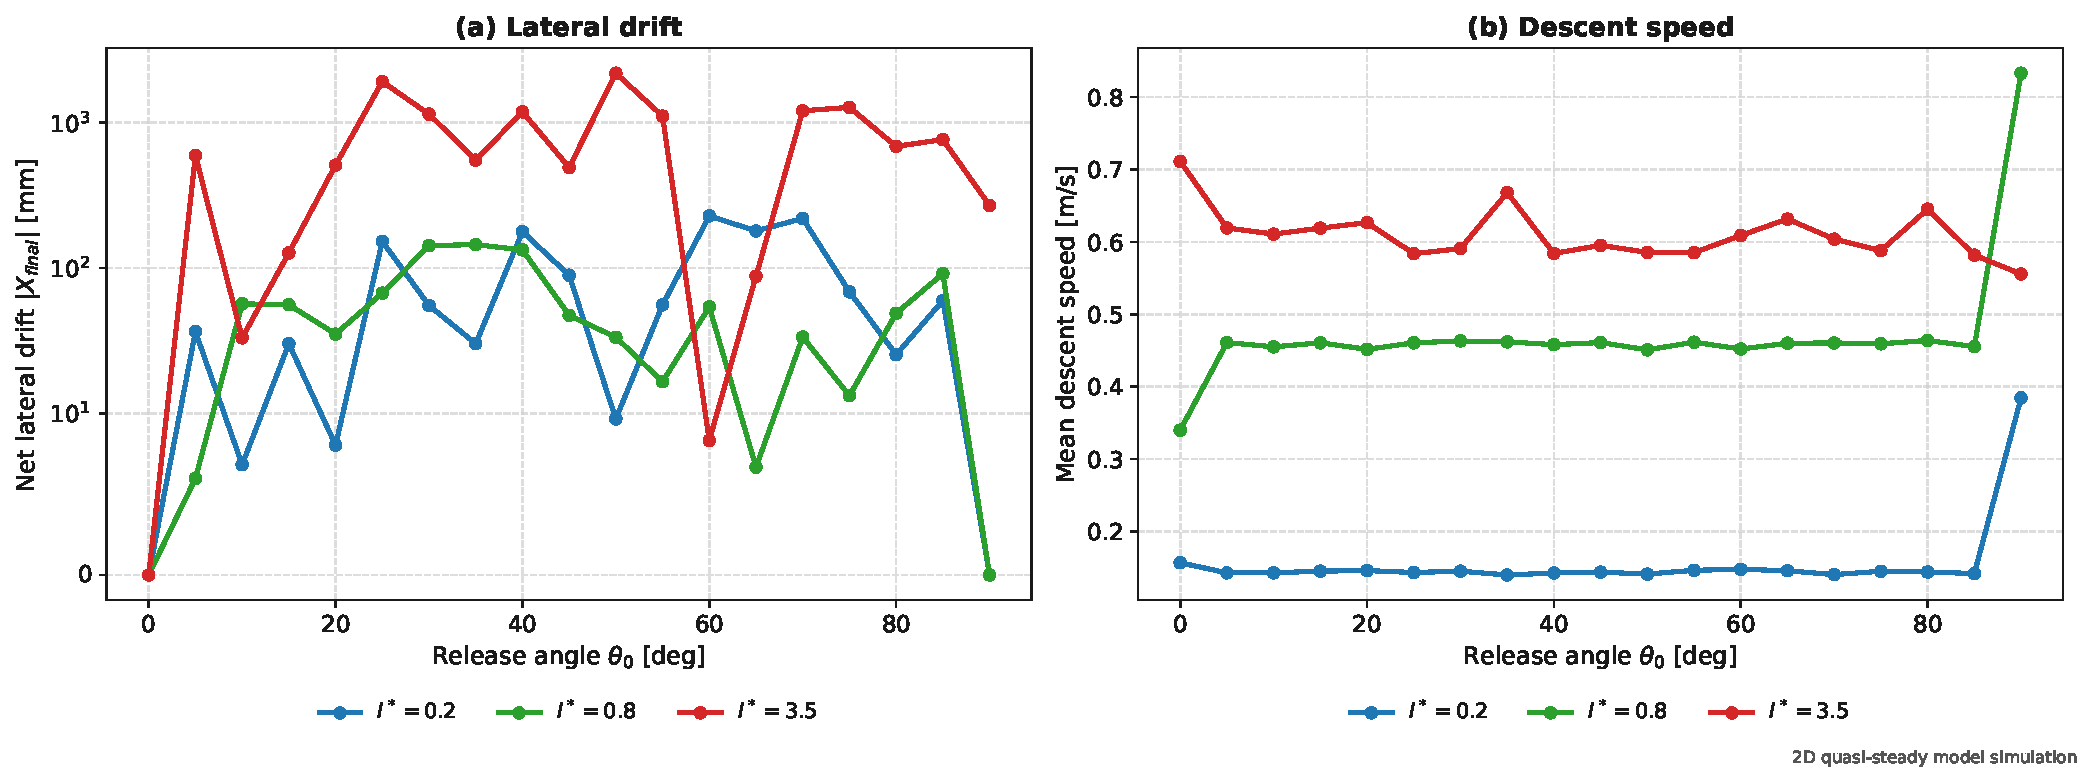
\includegraphics[width=\columnwidth]{../results/paper_figures/F09_release_angle_sweep.pdf}
    \caption{Initial release angle sensitivity across $\theta_0 \in [0^\circ, 90^\circ]$ (\texttt{F09\_release\_angle\_sweep}, 2D quasi-steady ODE simulation) for $I^* = 0.20, 0.80$, and $3.50$.}
    \label{fig:f09}
\end{figure}

\begin{figure}[t]
    \centering
    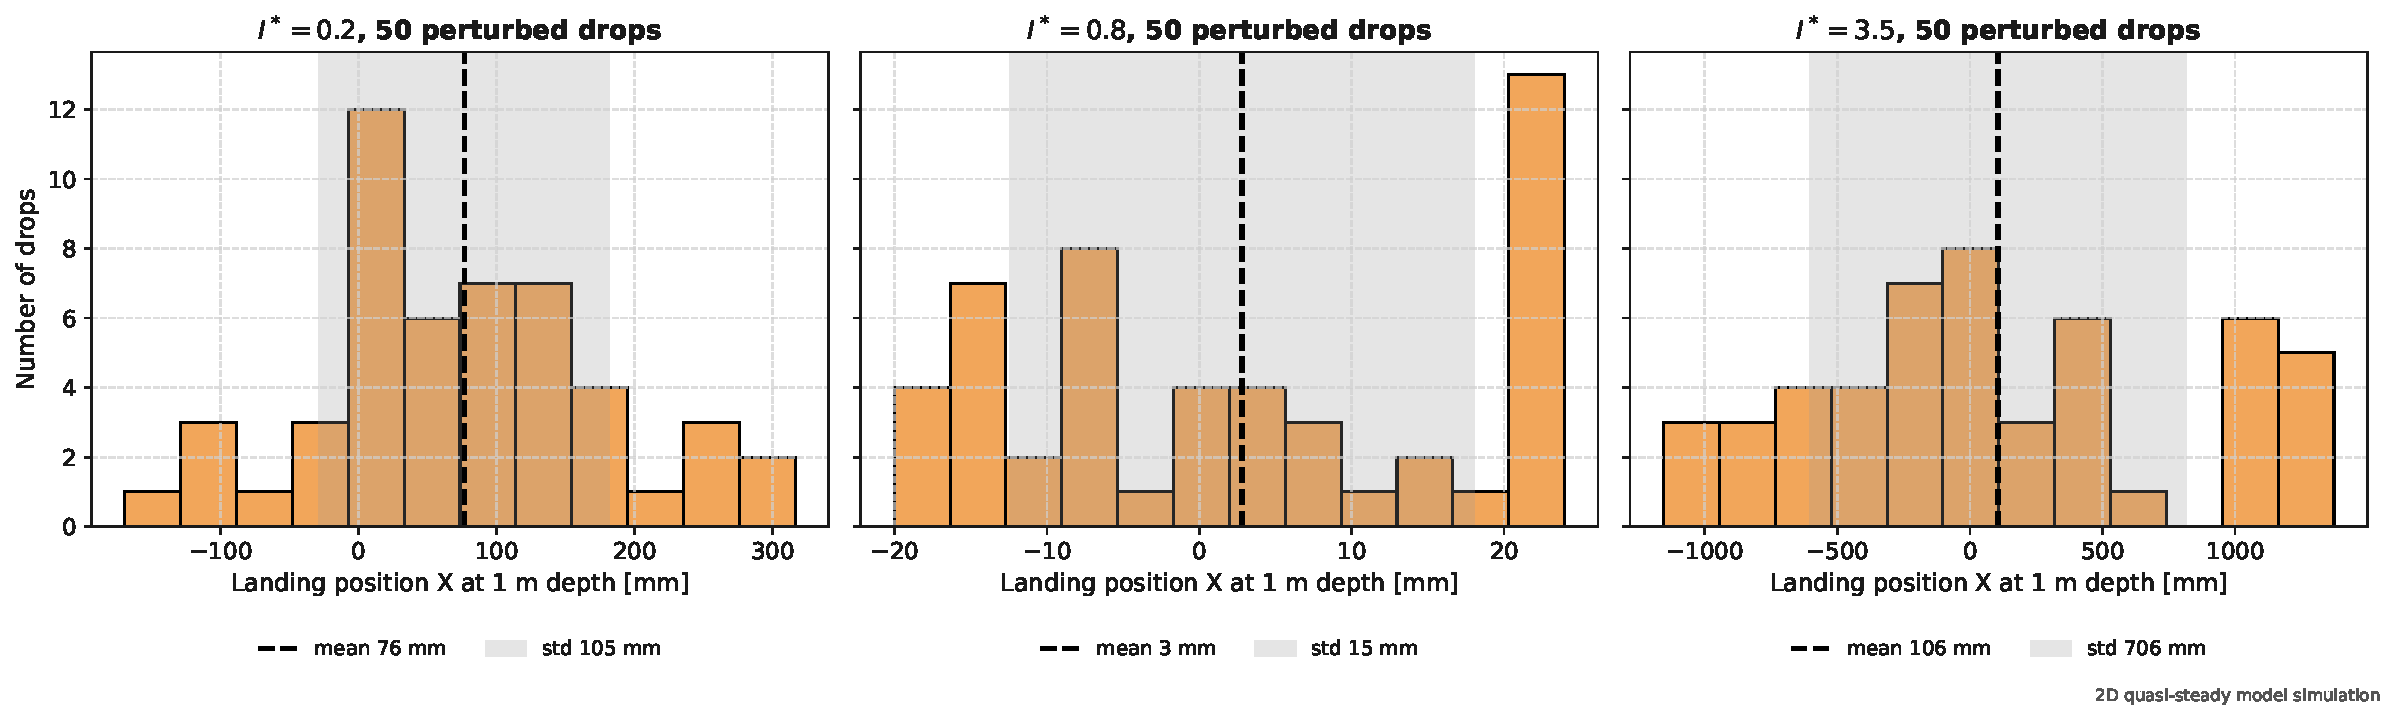
\includegraphics[width=\columnwidth]{../results/paper_figures/F10_landing_scatter.pdf}
    \caption{Landing dispersion histograms for 50-drop Monte Carlo ensembles (\texttt{F10\_landing\_scatter}, 2D quasi-steady ODE simulation) with $\sigma_\theta = 0.5^\circ$ and $\sigma_v = 10^{-4}\,\mathrm{m/s}$, showing the $46.52\times$ chaotic scatter amplification from $I^* = 0.80$ to $I^* = 3.50$.}
    \label{fig:f10}
\end{figure}

\begin{table}[t]
\centering
\caption{Monte Carlo landing dispersion statistics ($N = 50$ drops per case, $\theta_0 \sim \mathcal{N}(5^\circ, 0.5^\circ)$, $u_0, v_0 \sim \mathcal{N}(0, 10^{-4}\,\mathrm{m/s})$).}
\label{tab:chaos}
\footnotesize
\begin{tabular}{lccccr}
\toprule
\textbf{Case ($I^*$)} & $\langle X \rangle$ [mm] & $\sigma_X$ [mm] & Min / Max $X$ [mm] & Span [mm] & Ratio \\
\midrule
Low ($0.20$)  & $+76.47$  & $\mathbf{105.83}$ & $[-169.5, +316.3]$   & $485.8$  & $6.90\times$ \\
Mid ($0.80$)  & $+2.80$   & $\mathbf{15.34}$  & $[-20.0, +24.0]$     & $44.0$   & $1.00\times$ \\
High ($3.50$) & $+105.92$ & $\mathbf{713.64}$ & $[-1155.2, +1372.9]$ & $2528.0$ & $\mathbf{46.52\times}$ \\
\bottomrule
\end{tabular}
\end{table}

To quantify sensitivity to microscopic release noise, we executed 50-drop Monte Carlo ensembles at $I^* = 0.20, 0.80,$ and $3.50$ with Gaussian perturbations $\sigma_\theta = 0.5^\circ$ and $\sigma_v = 10^{-4}\,\mathrm{m/s}$ (Figure~\ref{fig:f10} and Table~\ref{tab:chaos}). At intermediate inertia ($I^* = 0.80$), rapid contraction onto the periodic limit cycle confines the landing footprint to a span of just $43.99\,\mathrm{mm}$ ($\sigma_X = 15.34\,\mathrm{mm}$) with a characteristic bimodal arcsine histogram corresponding to turnaround phase sampling. At high inertia ($I^* = 3.50$), trajectories repeatedly graze the heteroclinic separatrix between flutter and tumble, amplifying the landing standard deviation by $\mathbf{46.52\times}$ to $\sigma_X = 713.64\,\mathrm{mm}$ (spanning $2.528\,\mathrm{m}$).

\subsection{Catalog of Real-World \& Design Coins}
Figure~\ref{fig:f03} and Table~\ref{tab:coins} evaluate nine real-world and design coins across four release angles ($\theta_0 \in \{5^\circ, 20^\circ, 45^\circ, 90^\circ\}$) and both damping values ($\mu_1 = 0.20$ vs.\ $0.01$) in a $0.38\,\mathrm{m}$ tank. Pakistani circulation coins (\texttt{pk\_rs10} at $I^* = 0.4232$ and \texttt{pk\_rs5\_2002} at $I^* = 0.5999$) exhibit robust planar fluttering across all release angles. Notably, \texttt{design\_brass\_24x3.0} ($I^* = 1.0646$) lies between the $\mu_1 = 0.01$ threshold ($0.9703$) and the $\mu_1 = 0.20$ threshold ($1.2172$), switching completely from \texttt{fluttering} at $\mu_1 = 0.20$ to \texttt{tumbling} at $\mu_1 = 0.01$. Thicker brass (\texttt{design\_brass\_24x3.5}, $I^* = 1.2421$) tumbles robustly under both settings, while steel ($I^* = 1.4748$), lead ($I^* = 1.6571$), and tungsten ($I^* = 2.4111$) enter the chaotic \texttt{mixed} regime.

\begin{figure}[t]
    \centering
    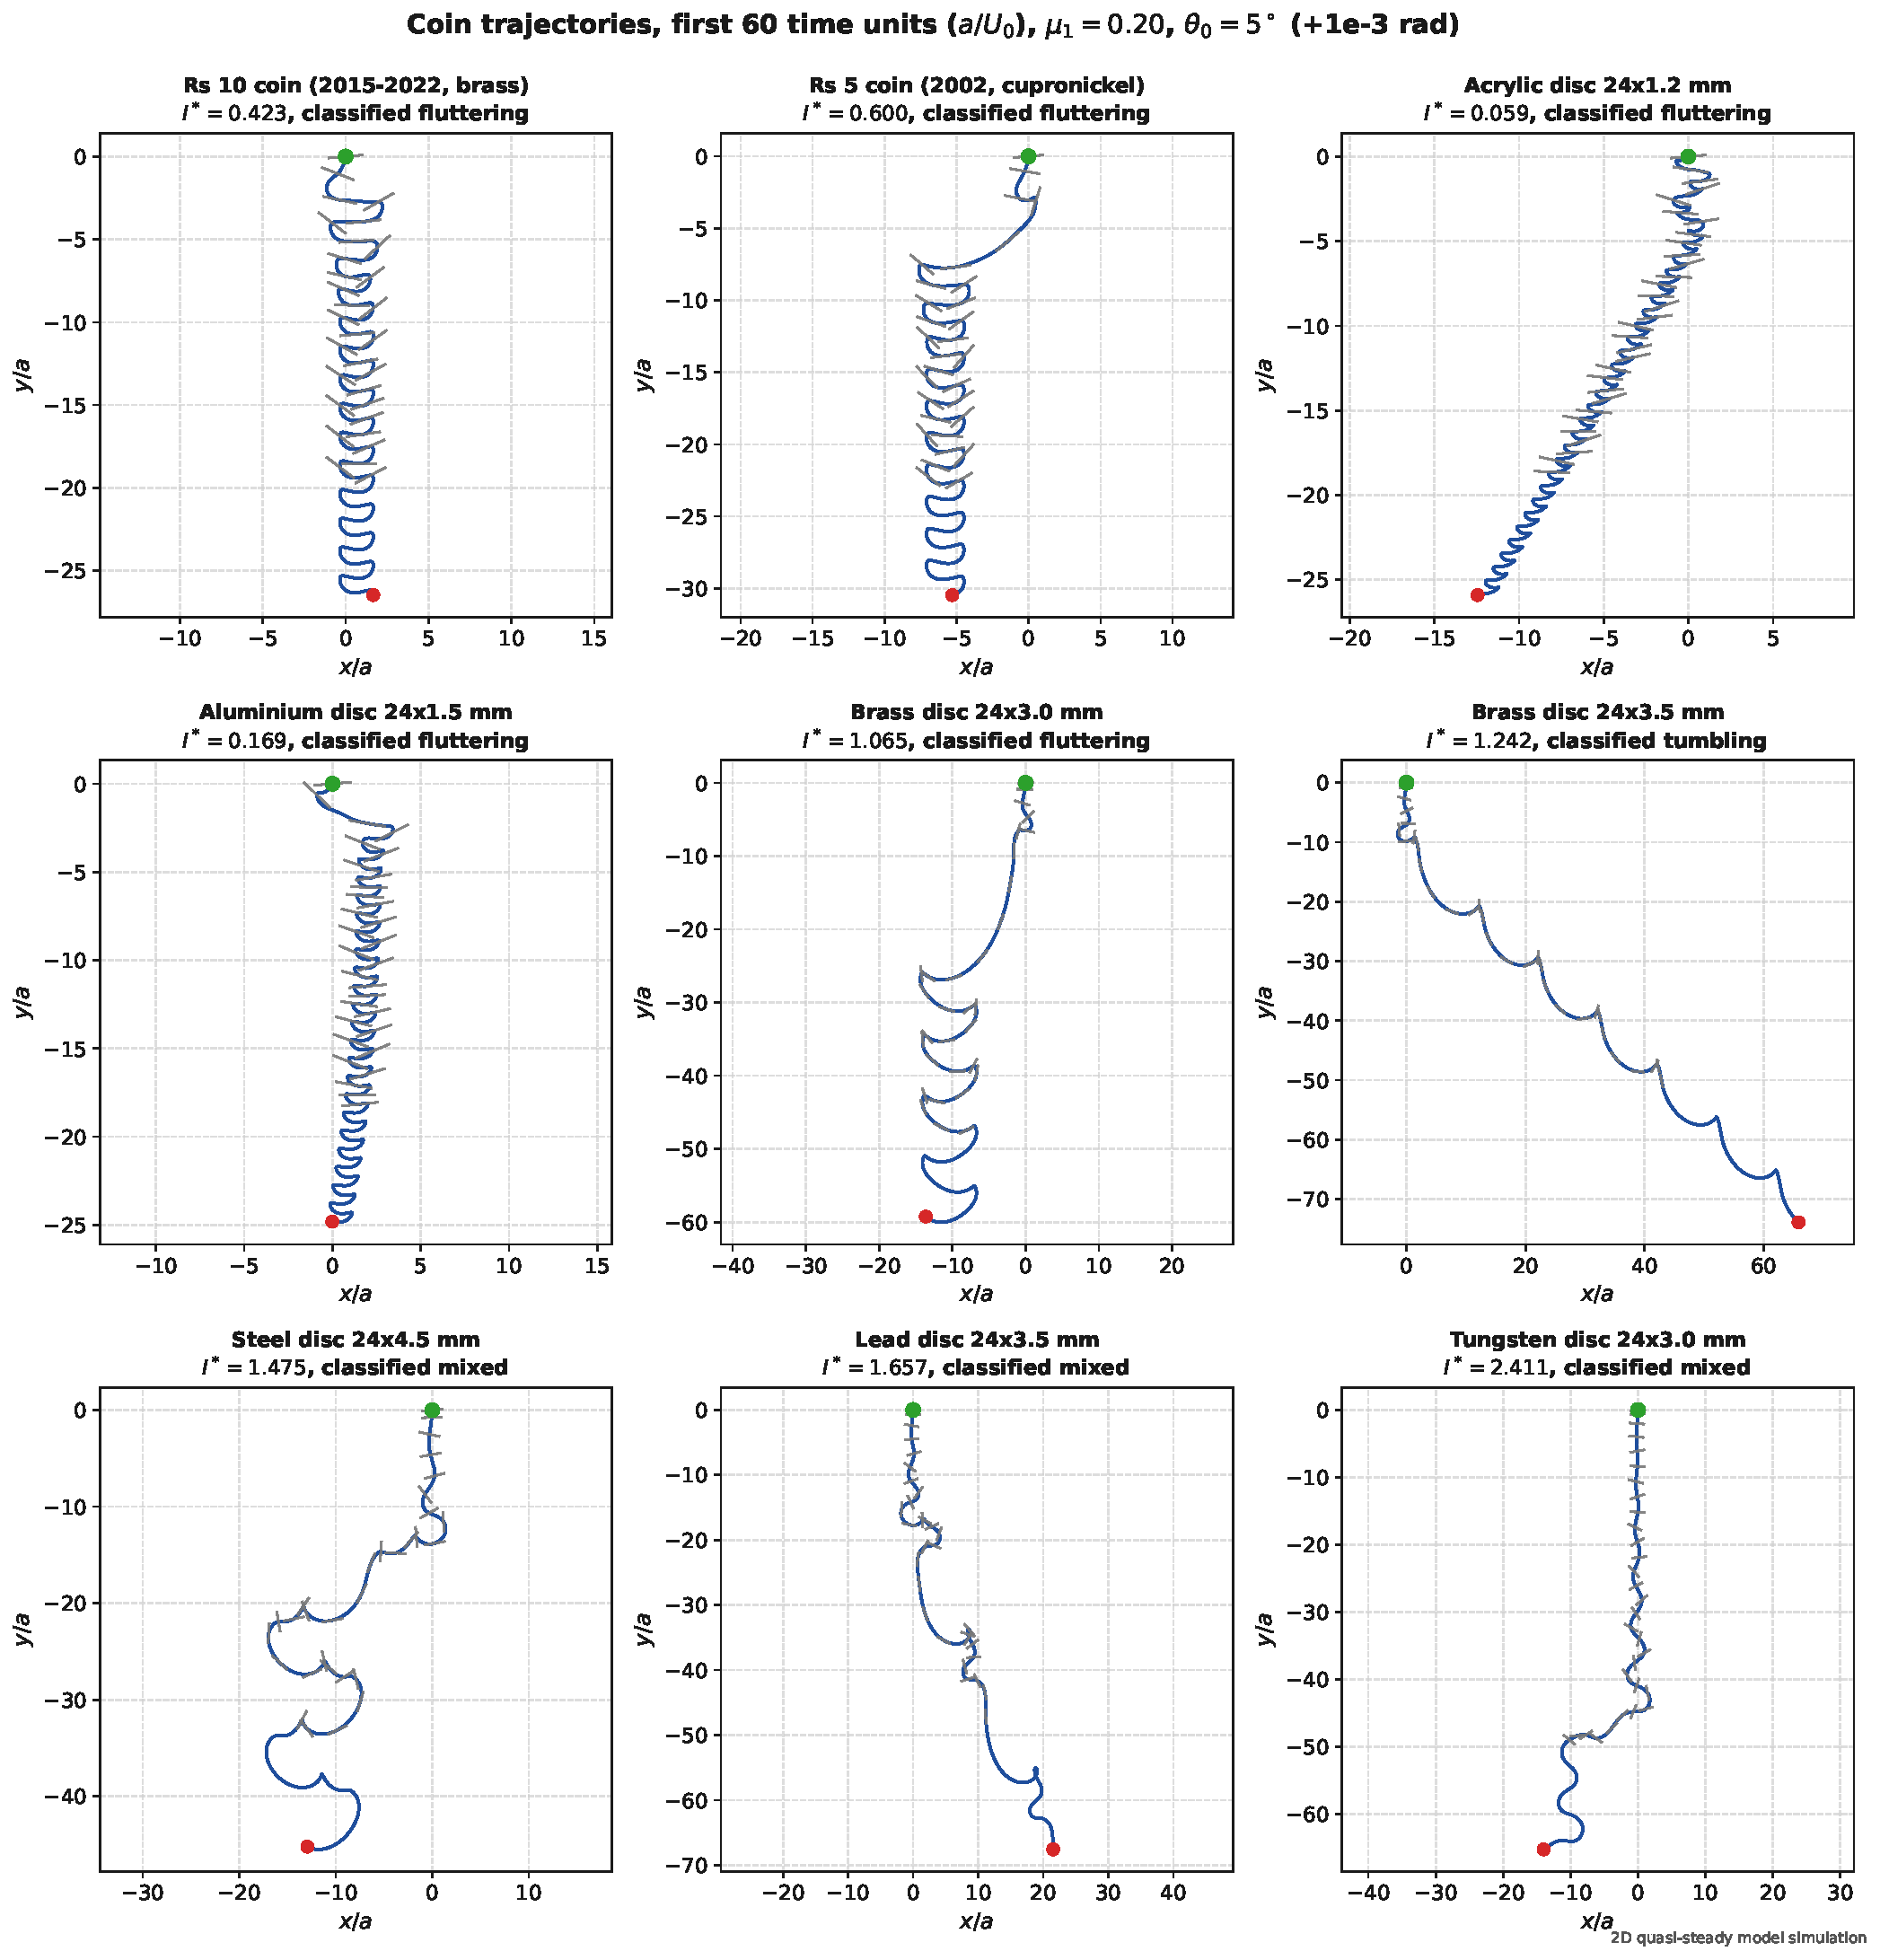
\includegraphics[width=\columnwidth]{../results/paper_figures/F03_coin_trajectories.pdf}
    \caption{Multi-panel catalog coin trajectories over a $0.38\,\mathrm{m}$ water tank depth (\texttt{F03\_coin\_trajectories}, 2D quasi-steady ODE simulation): (1) Pakistani Rs 10 ($I^*=0.423$, tight flutter), (2) Pakistani Rs 5 ($I^*=0.600$, moderate flutter), (3) Brass $24\times 3.5$ ($I^*=1.242$, unidirectional tumbling), and (4) Tungsten $24\times 3.0$ ($I^*=2.411$, mixed chaos).}
    \label{fig:f03}
\end{figure}

\begin{table}[t]
\centering
\caption{Regime classifications for the 9-coin catalog across $\theta_0 \in \{5^\circ, 20^\circ, 45^\circ, 90^\circ\}$ at baseline ($\mu_1 = 0.20$) vs.\ reduced ($\mu_1 = 0.01$) linear damping.}
\label{tab:coins}
\footnotesize
\begin{tabular}{lcccl}
\toprule
\textbf{Coin Identifier} & $I^*$ & $\rho_s/\rho_f$ & \textbf{Regime ($\mu_1=0.20$)} & \textbf{Regime ($\mu_1=0.01$)} \\
\midrule
\texttt{design\_acrylic\_24x1.2}   & $0.0591$ & $1.18$  & \texttt{fluttering} & \texttt{undetermined} ($5^\circ$) / \texttt{flutter} \\
\texttt{design\_aluminium\_24x1.5} & $0.1691$ & $2.71$  & \texttt{fluttering} & \texttt{fluttering} \\
\texttt{pk\_rs10}                  & $0.4232$ & $7.19$  & \texttt{fluttering} & \texttt{fluttering} \\
\texttt{pk\_rs5\_2002}             & $0.5999$ & $6.86$  & \texttt{fluttering} & \texttt{fluttering} \\
\texttt{design\_brass\_24x3.0}     & $1.0646$ & $8.52$  & \texttt{fluttering} & \texttt{tumbling} (All $\theta_0$) \\
\texttt{design\_brass\_24x3.5}     & $1.2421$ & $8.52$  & \texttt{tumbling}   & \texttt{tumbling} \\
\texttt{design\_steel\_24x4.5}     & $1.4748$ & $7.87$  & \texttt{mixed}      & \texttt{mixed} \\
\texttt{design\_lead\_24x3.5}      & $1.6571$ & $11.36$ & \texttt{mixed}      & \texttt{mixed} \\
\texttt{design\_tungsten\_24x3.0}  & $2.4111$ & $19.29$ & \texttt{mixed}      & \texttt{mixed} \\
\bottomrule
\end{tabular}
\end{table}

\subsection{Stage 2 Results: 2D WCSPH--FSI Comparison \& Explicit Viscosity Sweep}
Figures~\ref{fig:f11}, \ref{fig:f12}, and \ref{fig:f13} present the results of our C++20 2D WCSPH--FSI solver. Over the initial $0.35\,\mathrm{s}$ drop horizon (Figure~\ref{fig:f11}), the two-way coupled SPH plate qualitatively reproduces the initial Munk pitching onset and oscillation ranking across matched $I^*$ cases. Crucially, Figure~\ref{fig:f12} demonstrates what the fixed-coefficient ODE cannot: holding $I^* = 0.65$ fixed while varying dynamic viscosity $\mu$ across $\mathrm{Re} \in \{25, 100, 300, 800\}$ directly suppresses high-frequency pitching oscillations at low Reynolds number ($\mathrm{Re} = 25$), whereas higher Reynolds numbers ($\mathrm{Re} \ge 300$) sustain vortex-induced rocking.

\begin{figure}[t]
    \centering
    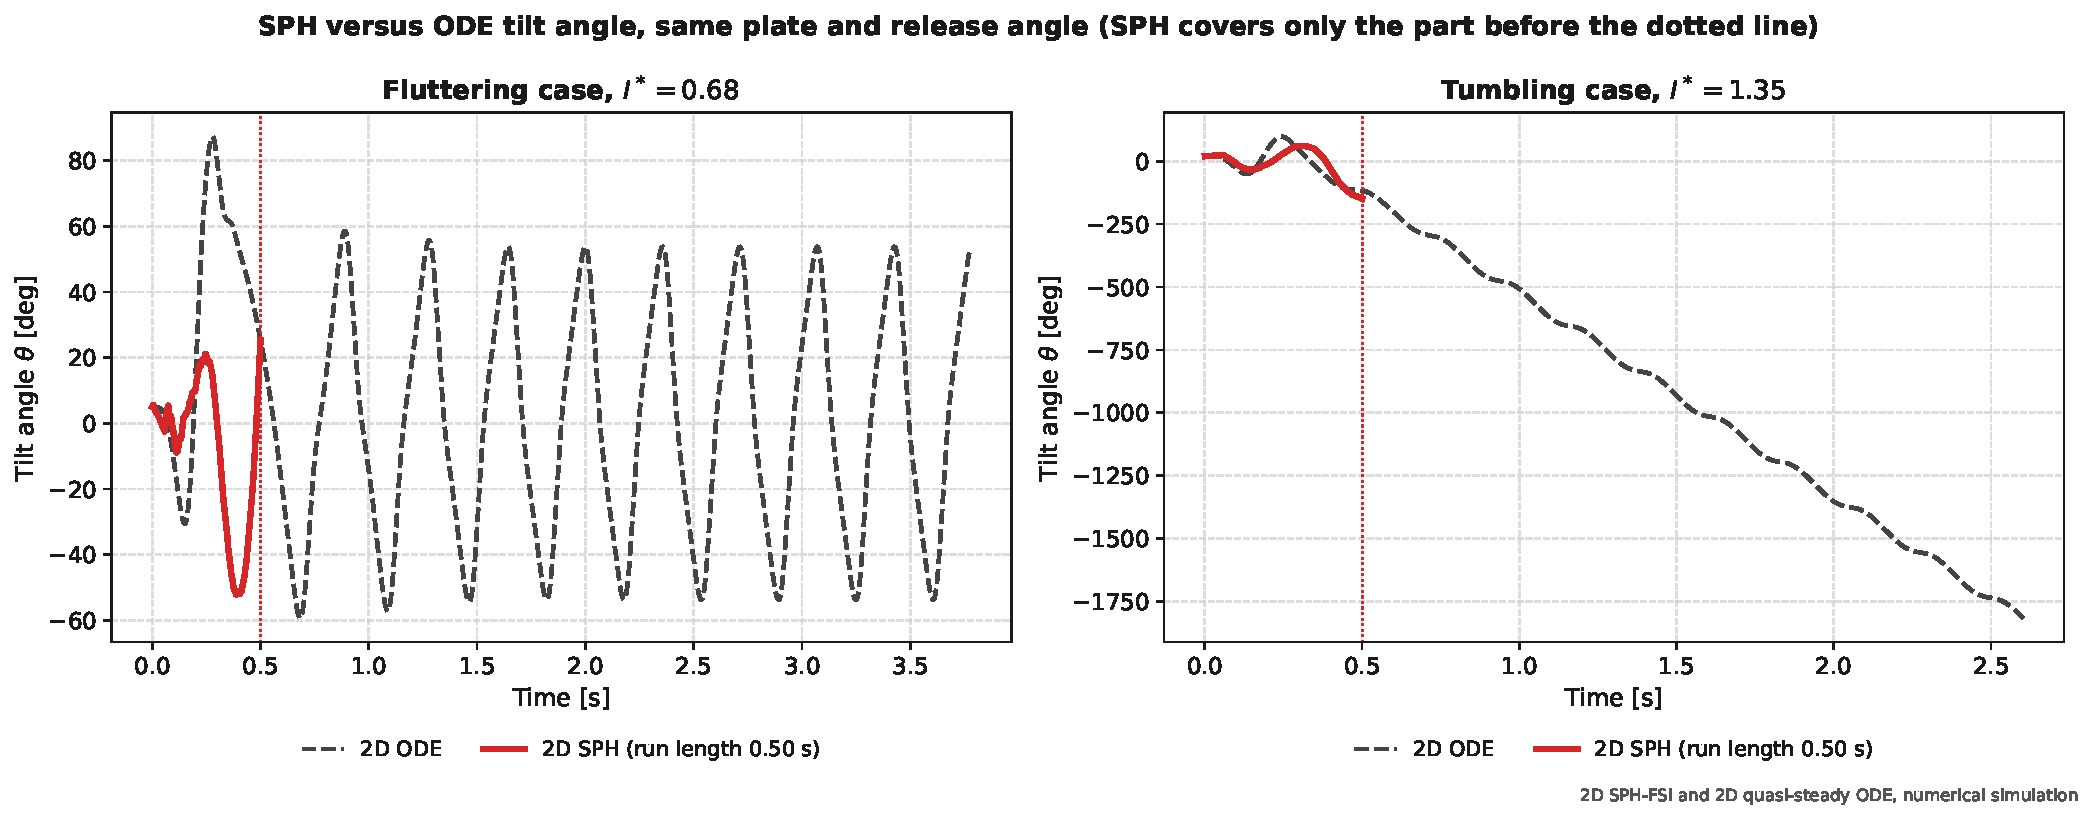
\includegraphics[width=\columnwidth]{../results/paper_figures/F11_sph_vs_ode_tilt.pdf}
    \caption{Direct time-history comparison of orientation tilt angle $\theta(t)$ between 2D WCSPH--FSI and the 2D quasi-steady ODE over the initial $0.35\,\mathrm{s}$ drop duration (\texttt{F11\_sph\_vs\_ode\_tilt}).}
    \label{fig:f11}
\end{figure}

\begin{figure}[t]
    \centering
    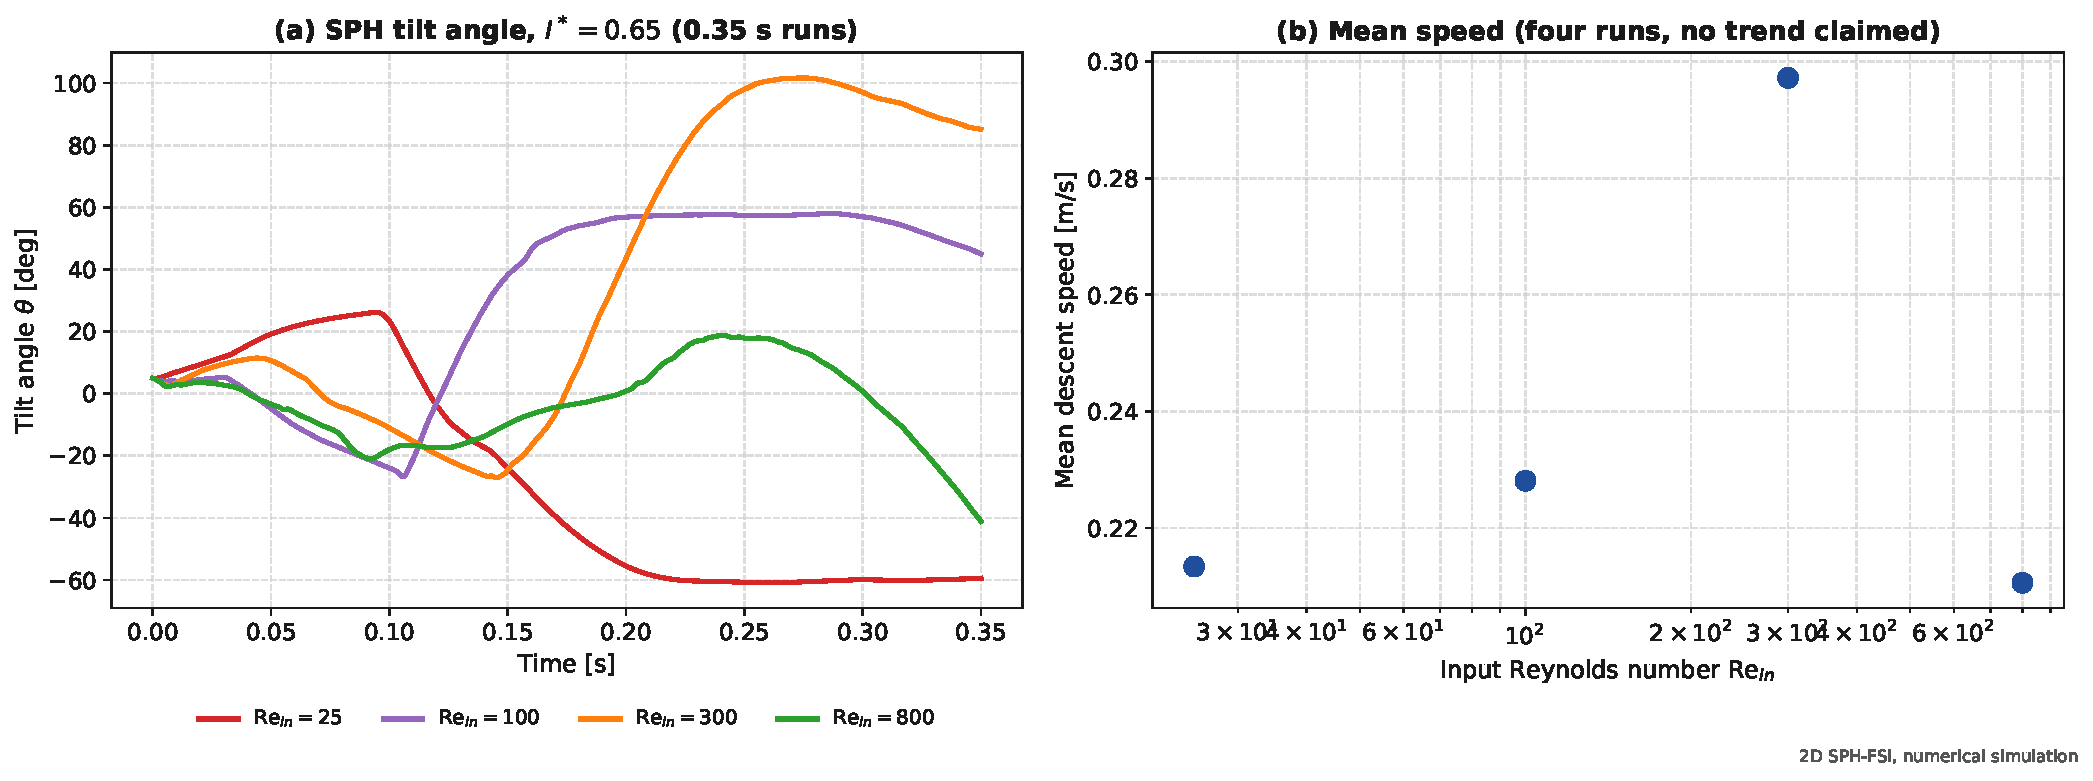
\includegraphics[width=\columnwidth]{../results/paper_figures/F12_sph_viscosity_sweep.pdf}
    \caption{2D WCSPH--FSI explicit viscosity sweep at fixed $I^* = 0.65$ across $\mathrm{Re} \in \{25, 100, 300, 800\}$ (\texttt{F12\_sph\_viscosity\_sweep}), showing viscous suppression of pitching at low $\mathrm{Re}$.}
    \label{fig:f12}
\end{figure}

\begin{figure}[t]
    \centering
    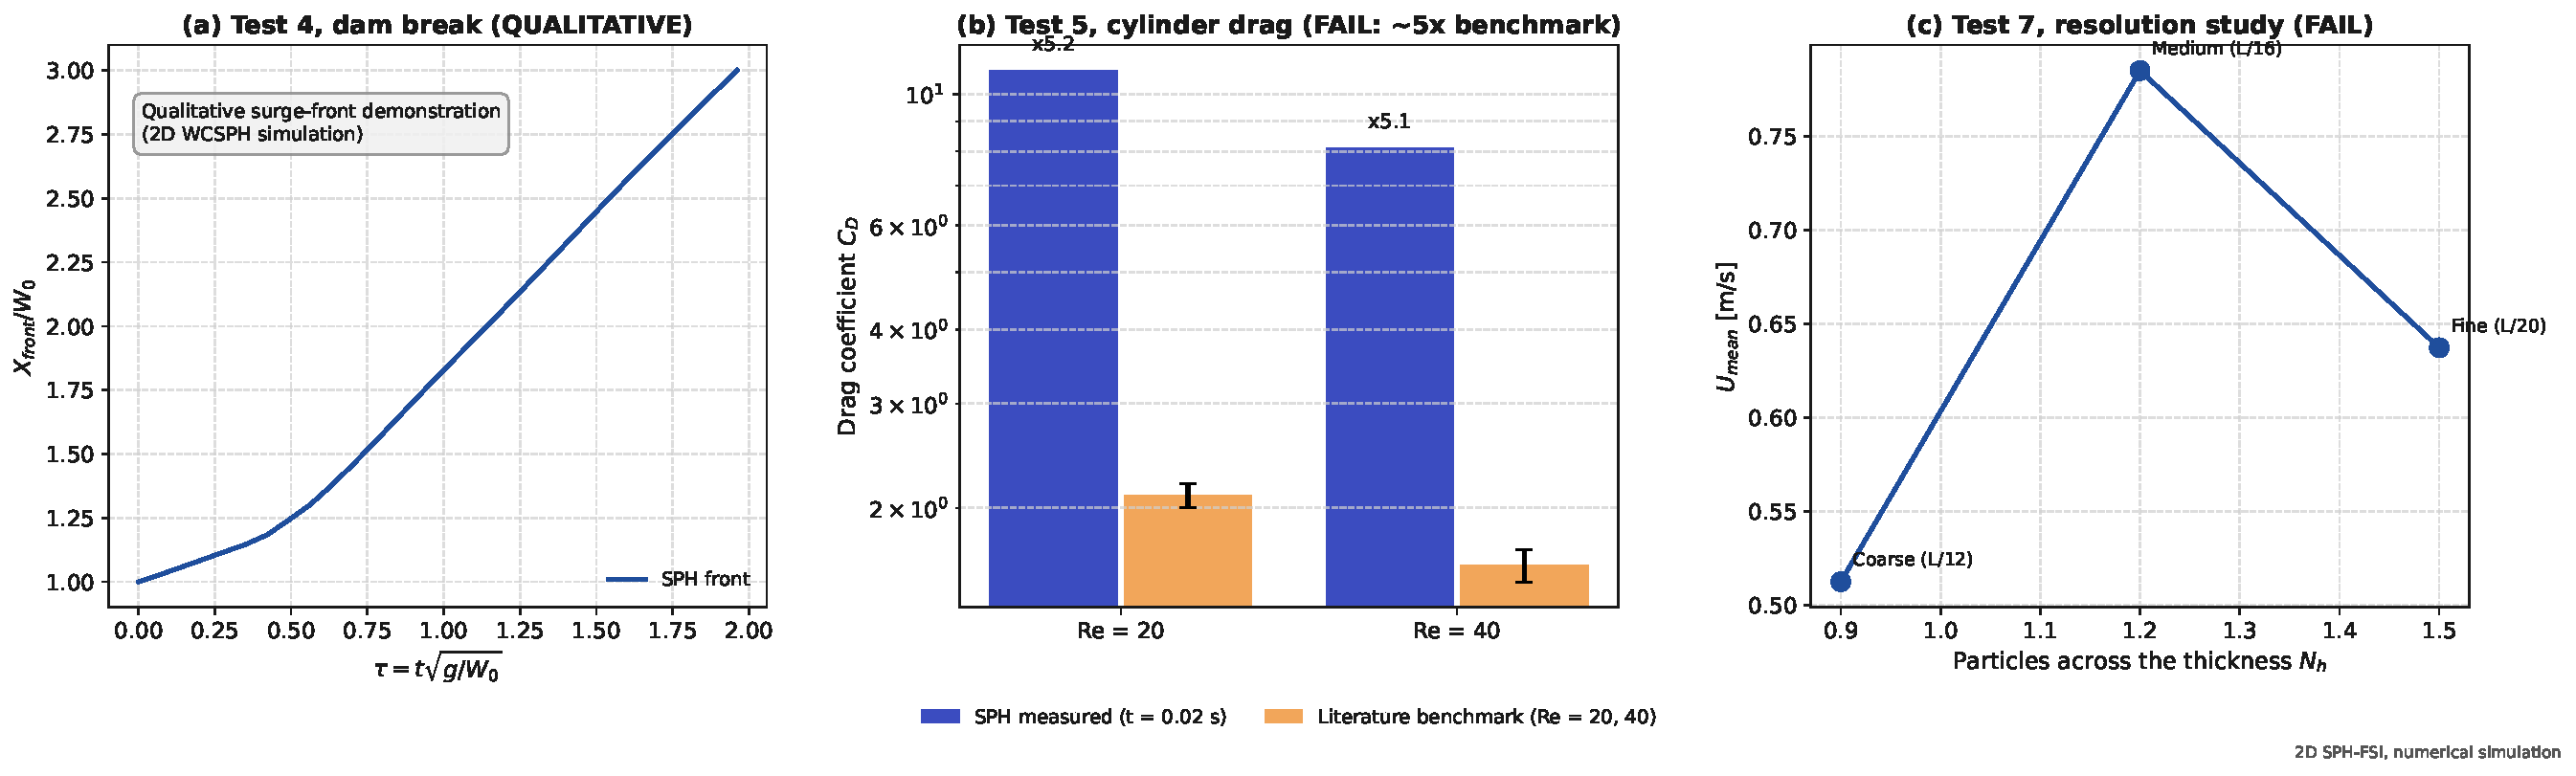
\includegraphics[width=\columnwidth]{../results/paper_figures/F13_sph_validation_problem_tests.pdf}
    \caption{SPH verification ladder diagnostic benchmarks (\texttt{F13\_sph\_validation\_problem\_tests}): (a) Test 4 dam-break surge front, (b) Test 5 cylinder drag showing the $5\times$ coarse-boundary-layer over-prediction at $\mathrm{Re}=20, 40$, and (c) Test 7 spatial grid convergence study ($\epsilon_{23} = 23.2\%$).}
    \label{fig:f13}
\end{figure}

\section{Literature Validation \& Model Limitations}
Figure~\ref{fig:f05} benchmarks our 2D ODE predictions against experimental literature:
\begin{enumerate}
    \item \textbf{Critical Inertia Threshold ($I^*_c$):} Our baseline prediction $I^*_c = 1.213 \pm 0.003$ agrees within $+1.08\%$ with the Andersen \textit{et al.} (2005b) experimental card transition midpoint $I^*_c = 1.20 \pm 0.10$ \cite{Andersen2005b}.
    \item \textbf{Strouhal Number ($\mathrm{St}$):} Across the fluttering regime, $\mathrm{St}$ decreases monotonically from $0.776$ ($I^* = 0.08$) and $0.394$ ($I^* = 0.39$) to $0.244$ ($I^* = 0.71$) and $0.154$ ($I^* = 0.87$), intersecting the Belmonte \textit{et al.} (1998) experimental strip band $\mathrm{St} \approx 0.18\text{--}0.22$ in the developed mid-flutter regime near $I^* \approx 0.75$ \cite{Belmonte1998}.
    \item \textbf{2D vs.\ 3D Descent Speed \& Stability Boundary:} Our 2D model predicts dimensionless descent speeds $U_{\mathrm{mean}}/U_t \approx 0.95$ ($I^* = 1.14$) and $0.79$ ($I^* = 1.38$), exceeding the experimental card values ($0.54$ and $0.62$) by $40\text{--}60\%$. Similarly, while our 2D model predicts that coins with $I^* \approx 0.42\text{--}0.60$ flutter, 3D stereo-tracked coin drops in the \texttt{ondrej-cloud} dataset (1 CZK, 5 CZK, 10 CZK) \cite{OndrejCloud} and Field \textit{et al.} (1997) \cite{Field1997} frequently exhibit 3D tumbling or chaotic coning at these inertia values. This difference arises because a 2D infinite-span strip lacks 3D tip-vortex induced drag and out-of-plane azimuthal pitching/yawing degrees of freedom, which destabilize planar flutter into 3D helical tumbling.
    \item \textbf{SPH Resolution Limits (Tests 5 \& 7):} As documented in Table~\ref{tab:verification} and Figure~\ref{fig:f13}, while our 2D WCSPH solver passes kernel consistency, hydrostatics, Archimedes buoyancy ($0.0012\%$ error), Couette shear ($0.23\%$), Taylor--Green vortex decay ($\nu_{\mathrm{meas}}/\nu = 0.9071$), and low-$I^*$ added-mass stability ($I^* = 0.05$), its coarse boundary discretization yields $C_D(20) = 10.96$ and $C_D(40) = 8.11$ ($\sim 5\times$ higher than DNS cylinder benchmarks) and a $23.2\%$ medium-to-fine grid difference in Test 7. Accordingly, the SPH results are strictly used for qualitative short-horizon FSI trends rather than DNS-grade drag predictions.
\end{enumerate}

\begin{figure}[t]
    \centering
    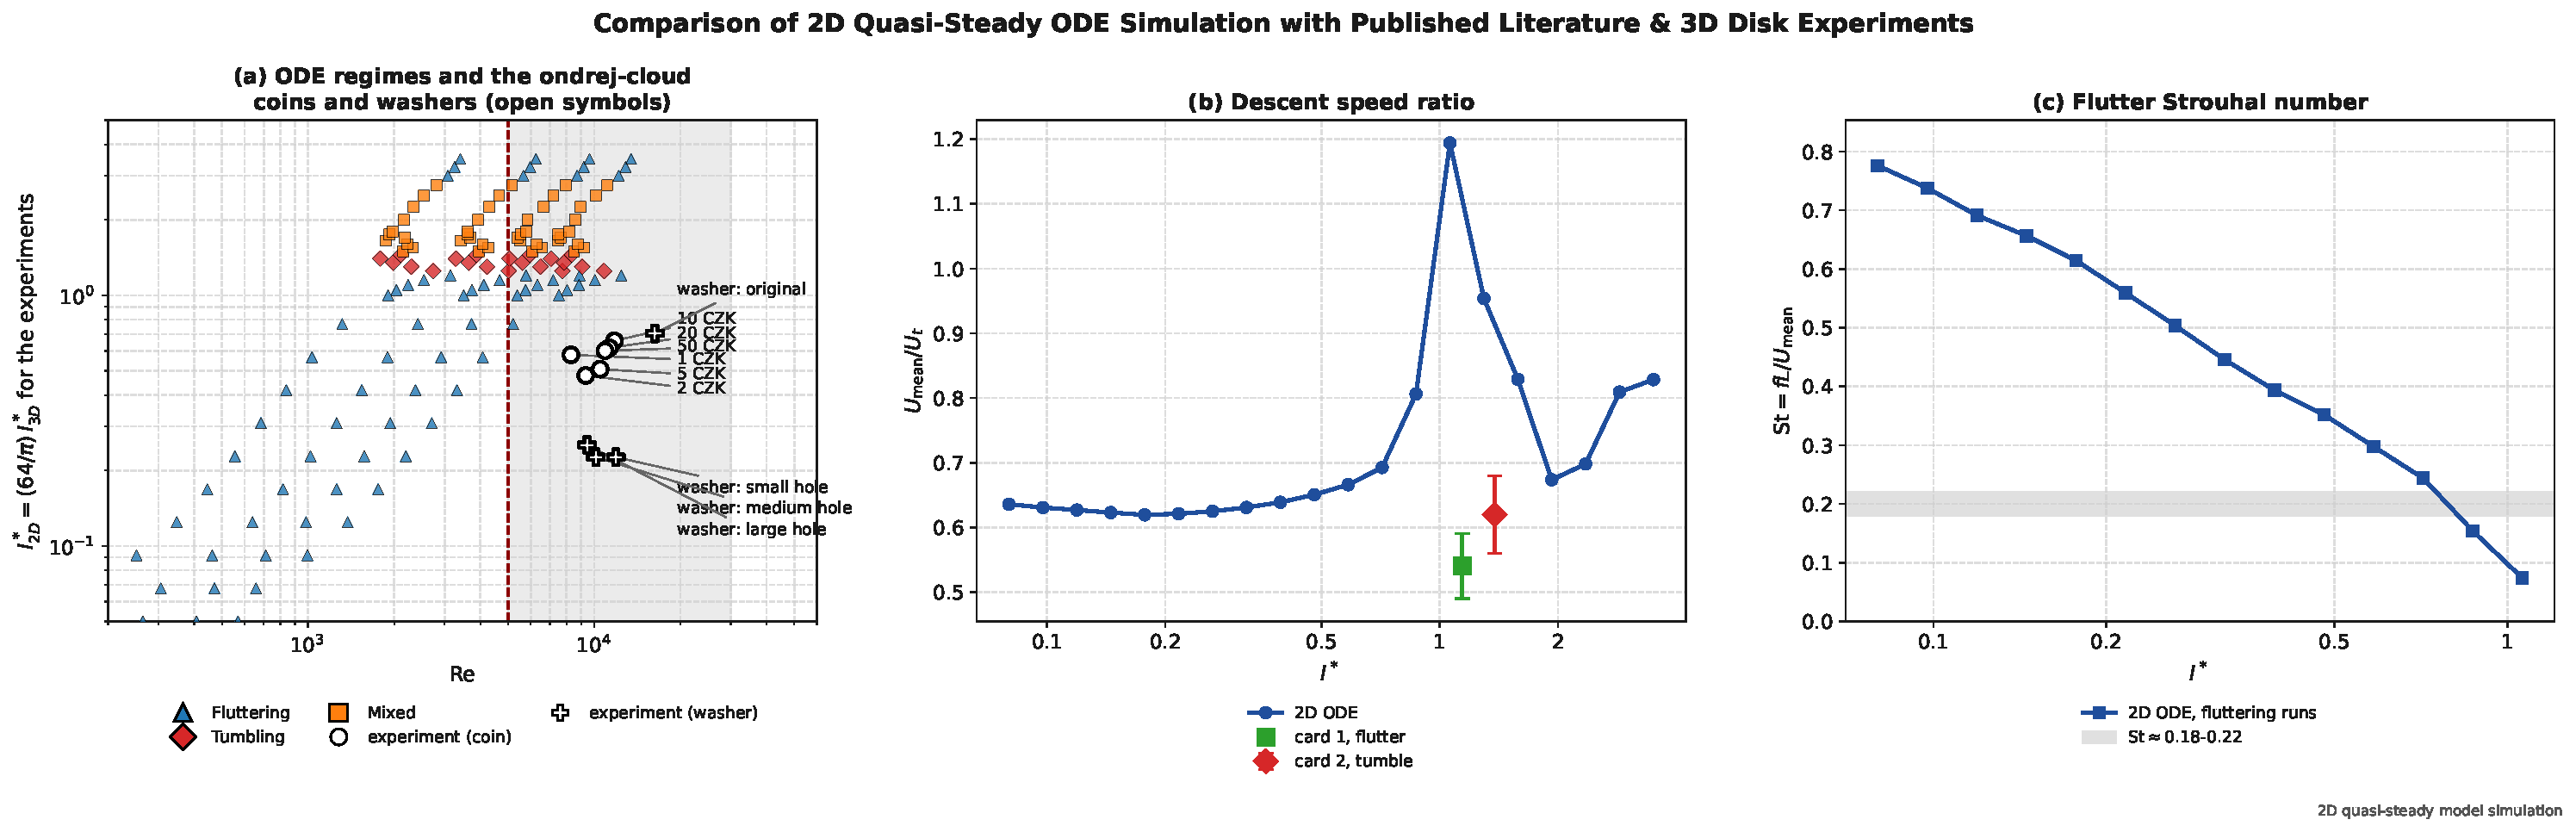
\includegraphics[width=\columnwidth]{../results/paper_figures/F05_literature_comparison.pdf}
    \caption{Quantitative validation against experimental literature (\texttt{F05\_literature\_comparison}, 2D quasi-steady ODE simulation): (a) dimensionless descent speed $U_{\mathrm{mean}}/U_t$ vs.\ Andersen \textit{et al.} (2005b) cards, and (b) Strouhal number $\mathrm{St} = fL/U$ vs.\ the Belmonte \textit{et al.} (1998) benchmark band $\mathrm{St} \approx 0.18\text{--}0.22$.}
    \label{fig:f05}
\end{figure}

\section{Conclusion}
We have established a fully verified two-stage computational framework for the ``Autumn Coin'' problem:
\begin{enumerate}
    \item \textbf{Dimensionless Inertia ($I^*$):} $I^* = (\rho_s h)/(\rho_f L)$ is the primary bifurcation parameter sorting falling coins into periodic fluttering ($I^* \le 1.25$), unidirectional tumbling ($1.25 \le I^* \le 1.45$, where lateral drift surges past $1.5\,\mathrm{m}$), and mixed chaos ($I^* \ge 1.50$).
    \item \textbf{Linear Rotational Damping ($\mu_1$):} Retaining the theoretical linear damping $\mu_1 = 0.20$ is essential to reproduce the experimental transition threshold ($I^*_c = 1.213 \pm 0.003$, $+1.08\%$ error vs.\ Andersen \textit{et al.}'s $1.20$ midpoint).
    \item \textbf{Perturbation Sensitivity \& Chaos:} Unperturbed steady descent is linearly unstable for coins in water ($0/136$ steady runs under $\Delta\theta = 10^{-3}\,\mathrm{rad}$), and crossing from the fluttering limit cycle ($I^* = 0.80$) into the chaotic regime ($I^* = 3.50$) amplifies landing scatter by $46.52\times$ ($\sigma_X = 15.34\,\mathrm{mm} \to 713.64\,\mathrm{mm}$).
    \item \textbf{Explicit Viscosity (2D WCSPH--FSI):} Direct SPH simulations confirm that high fluid viscosity ($\mathrm{Re} = 25$) damps pitching oscillations at fixed $I^* = 0.65$, while transparently establishing the resolution requirements for future 3D FSI extensions.
\end{enumerate}

\begin{thebibliography}{9}
\bibitem{Field1997} S. B. Field, M. Klaus, M. G. Moore, and F. Nori, ``Chaotic dynamics of falling disks,'' \textit{Nature} \textbf{388}, 252--254 (1997). \url{https://doi.org/10.1038/40817}
\bibitem{Belmonte1998} A. Belmonte, H. Eisenberg, and E. Moses, ``From flutter to tumble: Inertial drag and Froude similarity in falling paper,'' \textit{Phys. Rev. Lett.} \textbf{81}, 345--348 (1998). \url{https://doi.org/10.1103/PhysRevLett.81.345}
\bibitem{Pesavento2004} U. Pesavento and Z. J. Wang, ``Falling paper: Navier--Stokes solutions, model of fluid forces, and center of mass elevation,'' \textit{Phys. Rev. Lett.} \textbf{93}, 144501 (2004). \url{https://doi.org/10.1103/PhysRevLett.93.144501}
\bibitem{Andersen2005a} A. Andersen, U. Pesavento, and Z. J. Wang, ``Unsteady aerodynamics of fluttering and tumbling plates,'' \textit{J. Fluid Mech.} \textbf{541}, 65--90 (2005a). \url{https://doi.org/10.1017/S002211200500594X}
\bibitem{Andersen2005b} A. Andersen, U. Pesavento, and Z. J. Wang, ``Analysis of transitions between fluttering, tumbling and steady descent of falling cards,'' \textit{J. Fluid Mech.} \textbf{541}, 91--104 (2005b). \url{https://doi.org/10.1017/S0022112005005847}
\bibitem{Lamb1932} H. Lamb, \textit{Hydrodynamics}, 6th ed. (Cambridge University Press, Cambridge, 1932).
\bibitem{Morris1997} J. P. Morris, P. J. Fox, and Y. Zhu, ``Modeling low Reynolds number incompressible flows using SPH,'' \textit{J. Comput. Phys.} \textbf{136}, 214--226 (1997).
\bibitem{Akinci2012} N. Akinci, M. Ihmsen, G. Akinci, B. Solenthaler, and M. Teschner, ``Versatile rigid-fluid coupling for incompressible SPH,'' \textit{ACM Trans. Graph.} \textbf{31}(4), 62 (2012).
\bibitem{Adami2012} S. Adami, X. Y. Hu, and N. A. Adams, ``A generalized wall boundary condition for smoothed particle hydrodynamics,'' \textit{J. Comput. Phys.} \textbf{231}, 7057--7075 (2012).
\bibitem{OndrejCloud} O. \v{S}r\'{a}mek \textit{et al.}, ``autumn-coin: 3D stereo tracking and quasi-steady simulation of coins falling through water,'' GitHub repository (MIT License), \url{https://github.com/ondrej-cloud/autumn-coin}.
\end{thebibliography}

\end{document}
